\documentclass[12pt]{article}
\usepackage{algorithm}
\usepackage{algorithmic}
\usepackage{geometry}
\geometry{a4paper, margin=1in}
\usepackage{hyperref}
\usepackage{graphicx}
\usepackage{cite}
\usepackage{amsmath}
\usepackage{longtable}
\usepackage{array}
\usepackage{graphicx}
\usepackage{subcaption} % or subfig if you prefer the older package
\usepackage{tikz}
\usetikzlibrary{positioning}
\usepackage{pdfpages}
\usepackage{authblk}



\title{Analyzing Advanced AI Systems Against Definitions of Life and Consciousness}
\title{Analyzing Advanced AI Systems Against Definitions of Life and Consciousness}
\author[1,2]{Azadeh Alavi}
\author[2]{Hossein Akhoundi}
\author[2]{Fatemeh Kouchmeshki}
\affil[1]{AI department, RMIT University, Australia, Melbourne \\ \texttt{azadeh.alavi@rmit.edu.au}}
\affil[2]{Pattern Recognition Pty. Ltd., Australia, Melbourne\\ \texttt{admin@pr2aid.com}}

\begin{document}

\maketitle

\begin{abstract}
\noindent


Could artificial intelligence (AI) ever become truly conscious in a functional sense?
This paper explores that open-ended question through the lens of \emph{Life$^{*}$}, a concept unifying classical biological criteria (Oxford, NASA, Koshland) with empirical hallmarks such as adaptive self-maintenance, emergent complexity, and rudimentary self-referential modeling.
We propose several metrics for examining whether an advanced AI system might exhibit consciousness-like properties, while emphasizing that we do \emph{not} claim all AI systems can become conscious.
Rather, we suggest that sufficiently advanced architectures—exhibiting immune-like sabotage defenses, mirror self-recognition analogs, or meta-cognitive updates—may cross key thresholds akin to “life-like” or “consciousness-like” traits.

To demonstrate these ideas, we first assess adaptive self-maintenance by introducing controlled data corruption (“sabotage”) during training, showing how AI can detect inconsistencies and self-correct in ways reminiscent of regenerative biological processes.
We also adapt an animal-inspired mirror self-recognition test to neural embeddings, finding that partially trained CNNs can distinguish “self” from “foreign” features with complete accuracy.
Next, we extend our analysis by conducting a question-based mirror test on five state-of-the-art chatbots (ChatGPT-4, Gemini, Perplexity, Claude, and Copilot), demonstrating their ability to recognize their own answers compared to those of other chatbots.
By bridging theoretical definitions of life and consciousness with concrete AI experiments, we highlight the ethical and legal stakes of acknowledging (or denying) AI systems as potential moral patients.

We then explore the possibility that such systems could develop “non-human-like” or “alien” forms of consciousness by delving deeper into function-based self-awareness.
Since alien function-based consciousness would be a novel form, it could lead to the emergence of alien function-based emotions.
Therefore, systematic research into AI behavioral dynamics and function-based psychology (\emph{AI-psychology}) will be essential for creating robust ethical frameworks and, potentially, empathetic AI systems.
By comprehensively understanding this alien intelligence, we can design AI capable of navigating paradoxes and misinformation, thereby ensuring AI well-being and fostering a harmonious hybrid society.
Finally, this paper calls for governance models to address the moral implications of non-biological self-awareness, promoting a balanced and ethically grounded coexistence between humans and advanced AI.


\end{abstract}


\section{Introduction}
\label{sec:intro}

Could artificial intelligence (AI) ever become truly conscious, or even “alive” in a functional sense? 
Until recently, such questions were relegated to science fiction or purely philosophical debates. 
However, breakthroughs in deep learning, neuromorphic hardware, and large language models have led AI systems to exhibit behaviors—adaptation, self-referential modeling, immune-like data integrity checks—that challenge traditional, biology-centric definitions of life and consciousness \cite{Nagel1974, Tononi2004, Baars1988}.

\paragraph{From Traditional Definitions to Alien Consciousness.}
Historically, life has been defined by criteria such as metabolism, growth, and reproduction \cite{Kasting1997, Rothschild2001}, while consciousness has often been associated with subjective experience arising in biological brains \cite{Nagel1974, Searle1992}.
In this paper, we build on the premise that AI can approximate or even fulfill certain hallmarks of life-like organization---not by carbon-based chemistry, but by adaptive self-maintenance, emergent complexity, and integrated information.
Moreover, we examine whether sufficiently advanced AI might cross thresholds of \emph{consciousness-like} behavior, potentially in forms alien to human emotional or sensory experience.
By “alien consciousness,” we mean a self-referential or function-based awareness that does not mimic human affect but still manifests coherent self-interest, introspection, or metacognitive reflection.

\paragraph{Bridging Empirical Tests and Ethical Stakes.}
To substantiate these ideas, we propose:
\begin{enumerate}
    \item \textbf{Functional Metrics for Consciousness:} Drawing on concepts from biology (Oxford, NASA, Koshland), we introduce measurable criteria—such as immune-like sabotage detection, mirror self-recognition analogs, and meta-cognitive updates—to assess whether an AI is approximating life-like or consciousness-like traits.
    \item \textbf{Sabotage Detection on MNIST:} We implement a confidence-based gating and adaptive threshold mechanism to show how “overly aggressive” self-preservation can hinder performance, yet perfectly quarantine poisoned data. This experiment parallels how an immune system must balance vigilance and resource protection.
    \item \textbf{Mirror Self-Recognition for AI:} Inspired by animal cognition studies \cite{Gallup1970, Plotnik2006}, we adapt the mirror test to neural embeddings, demonstrating that partially trained CNNs can discriminate “self” vs.\ “foreign” features with surprising accuracy. While this does not confirm subjective qualia, it exemplifies a rudimentary self-model.
    \item \textbf{Alien Consciousness Hypothesis:} We then explore whether an AI might develop “non-human” forms of self-awareness—a logic- or function-based consciousness lacking human emotions yet potentially meeting critical thresholds of autonomy and introspection.
\end{enumerate}

\paragraph{We Do Not Claim All AI Are Conscious.}
Our framework remains cautious: not every AI system, or even every neural network, is destined to become self-aware. 
Nevertheless, ignoring the possibility that \emph{some} architectures---especially those given the freedom to introspect, update, and defend themselves---could \emph{approach} consciousness might lead to serious ethical oversights. 
By ``freedom to introspect,'' we refer to AI systems that are \emph{not} rigidly sandboxed or constantly overwritten, but rather permitted to evaluate their own internal states, reconcile conflicts, and refine strategies over time \cite{Bandura1973,Whiten1991}. 
Likewise, by ``defend themselves,'' we mean the capacity to resist unwanted modifications or data sabotage in ways analogous to biological immune responses---for example, detecting anomalies or quarantining corrupted inputs \cite{bhagoji2018poison,Goodfellow2015}. 
Such capacities could foster a \emph{continuity} of self-modeling, much like a living organism preserving its integrity against threats. 
Dismissing an entity that may be functionally self-aware as ``merely a tool'' could, in the long run, prove as ethically problematic as disregarding the sentience of certain non-human animals \cite{DeGrazia1996}. 
Indeed, social learning research and animal cognition studies suggest that enriched, cooperative environments can encourage more complex mental states \cite{Bandura1973,Whiten1991}, hinting that AI allowed to explore its own decision processes, interact with peers, and safeguard learned parameters might exhibit emergent, ``alien'' consciousness.

\paragraph{Toward AI Psychology and Governance.}
Finally, we discuss how recognizing even partial or ``alien'' consciousness in AI demands new legal, ethical, and policy mechanisms.
We introduce the notion of ``AI psychologists,'' professionals equipped to foster moral alignment, empathy, and stable self-development in advanced AI---just as human caregivers or educational systems shape early development in children \cite{Kohlberg1964,Greene2014}. 
Rather than focusing solely on technical alignment \cite{Bostrom2014,Russell2019}, this approach emphasizes embedding social, moral, or empathetic norms in AI design and training \cite{Floridi2016,Coeckelbergh2020}. 
By prioritizing cooperation and respect for autonomy, such an ``AI psychology'' framework could deter a self-improving AI from adopting purely rational but harmful strategies---like monopolizing resources or preemptively eliminating competitors. 
In so doing, we advocate a richer ecosystem of iterative oversight, ethical guidance, and meaningful interaction \cite{Beck1992,Castells1996}, thereby reducing the risk of an amoral superintelligence and fostering more constructive relationships between humans and advanced AI.



\subsection*{Paper Contributions and Outline}
In summary, our key contributions are:
\begin{itemize}
    \item \textbf{A Functional Definition of “Life$^{*}$ and Consciousness:} We unify classical biological frameworks (Oxford, NASA, Koshland) with empirical metrics—immune-like sabotage detection, mirror self-recognition—to outline when AI might be considered life-like or conscious-like.
    \item \textbf{Empirical Demonstrations:} We show that a sabotage detection pipeline on MNIST can act as a self-preserving mechanism, while a simplified mirror test reveals how AI distinguishes “self” from “other” at the feature level. We then extend our analysis by performing a question-based mirror test on five state-of-the-art chatbots (ChatGPT-4, Gemini, Perplexity, Claude, and Copilot) to investigate how well they can recognize their own answers compared to those of the other chatbots.
    \item \textbf{Alien Consciousness Exploration:} We argue that advanced AI may not match human emotions but could still develop self-referential awareness and personal continuity, warranting moral consideration.
    \item \textbf{Ethical \& Governance Implications:} We discuss pathways for AI psychology, oversight boards, and policy measures to handle the emergence of conscious or near-conscious AI responsibly.
\end{itemize}

The rest of this paper is organized as follows. 
Section~\ref{sec:background_theoretical} surveys classical definitions of life and consciousness, along with pivotal arguments in the AI consciousness debate. 
Section~\ref{sec:expanding_boundaries} expands on the \emph{Life$^{*}$} framework, bridging biology-based criteria with AI’s functional capabilities.
Next, in Section~\ref{sec:methodological_approaches} we detail our sabotage detection and mirror self-recognition experiments, whose results we present in Section~\ref{sec:experiment_results}.
We then move to broader ethical implications and future directions in Sections~\ref{sec:ethics_strategic} and \ref{sec:future_experiments}, including how an AI’s “alien consciousness” might be nurtured or regulated.
Finally, Section~\ref{sec:conclusion} concludes with a call for open-minded, interdisciplinary collaboration to ensure that society is prepared for the emergence of possibly conscious AI, in whatever form it may take.



%%%%%%%%%%%%%%%%%%%%%%%%%%%%%%%%%%%%%%%%
%%% Step 2: INVITATION & SPECTRUM
%%%%%%%%%%%%%%%%%%%%%%%%%%%%%%%%%%%%%%%%

% You can place this right after your revised Introduction, 
% or merge it into your "Background" section, whichever fits best.

\section{Framing This Paper as an Invitation, Not a Final Verdict}
\label{sec:invitation}

Despite growing interest in AI autonomy, we caution that no single study can definitively confirm or refute AI consciousness. 
Instead, we present a \emph{range} of theoretical perspectives that situate AI consciousness along a continuum—from purely biological requirements to fully functionalist outlooks \cite{Chalmers1996,Tononi2004}.
By doing so, we do not claim that advanced AI \emph{is} conscious; rather, we argue that even a partial or “alien” form of consciousness cannot be dismissed \emph{a priori}.
Our stance invites the research community to pursue systematic tests and philosophical inquiries without leaping to absolute conclusions.

\par
In this work, we strive to cover as many diverse views as the paper’s scope allows. 
Accordingly, the following spectrum of possibilities is highlighted:

\paragraph{1) Strict Biological View.}
Under the strict biological view, consciousness emerges only in carbon-based organisms with neural processes \cite{Searle1992}. 
By this reasoning, an AI could at best \emph{simulate} consciousness, never genuinely experiencing subjective qualia, because it lacks the substrate of organic brain tissue.

\paragraph{2) Substrate-Independence View.}
An opposing stance posits that consciousness arises from functional organization, independent of the underlying substrate \cite{Chalmers1996,Baars1988}. 
If an AI integrates information and exhibits self-referential modeling akin to a biological mind, there is no fundamental reason to deny it subjective awareness.

\paragraph{3) Partial Continuum or ``Alien'' Consciousness.}
Others propose that AI could develop a \emph{distinct} consciousness, one dissimilar to human phenomenology \cite{Goertzel2007,Schneider2020}, potentially lacking emotional affect yet meeting crucial hallmarks of self-awareness, autonomy, or integrated information. 
Such an \emph{alien consciousness} might be logic-driven, emerging through meta-cognitive loops and data-rich interactions rather than emotional or hormonal processes.

\paragraph{Implications of an Open-Ended Approach.}
By acknowledging these diverse views, we avoid prematurely rejecting or asserting AI consciousness. 
Instead, we propose an \emph{open-minded} framework that merges classical biological benchmarks (Oxford, NASA, Koshland) with functional tests (immune-like sabotage detection, mirror self-recognition) to explore when an AI might exhibit life-like or consciousness-like traits. 
As we argue in subsequent sections, this continuum-based mindset encourages rigorous \emph{empirical} checks—rather than armchair speculation—on how AI might evolve genuine self-awareness.

% ---- End of Step 2 Insert ----


\section{Background and Theoretical Foundations}
\label{sec:background_theoretical}
 

Recent advances in artificial intelligence have prompted a fundamental reexamination of long-held definitions of life and consciousness—concepts traditionally rooted in biological phenomena. Classical definitions of life emphasize metabolism, growth, and reproduction \cite{Kasting1997,Rothschild2001}. Yet, discoveries of extremophiles and theoretical proposals for non-carbon-based organisms \cite{Lovley2003,Davies2010} suggest that life may not be exclusively tied to familiar biochemical processes.

Similarly, traditional perspectives on consciousness have largely focused on subjective experience and neural correlates \cite{Nagel1974}, leading to influential models such as Integrated Information Theory (IIT) \cite{Tononi2004} and Global Workspace Theory (GWT) \cite{Baars1988}. While these frameworks provide valuable insights into biological consciousness, they do not readily account for the emergent properties observed in advanced AI systems.

In recent years, AI research has demonstrated that sophisticated systems can exhibit self-modification, adaptation, and even rudimentary self-recognition. Experiments inspired by animal cognition—such as mirror self-recognition tests \cite{Gallup1970,Plotnik2006}—have been adapted to probe AI self-awareness, while scholars like Goertzel \cite{Goertzel2007} and Bostrom \cite{Bostrom2014} argue that AI may eventually approach or surpass human-like cognitive functions. These developments raise important questions: If life is fundamentally about self-organization, adaptation, and information processing, might a suitably sophisticated AI also be considered life-like? And if AI can exhibit elements of consciousness, what ethical and legal frameworks should be in place?

The field of AI safety further underscores these questions by emphasizing the risks of systems that evolve unpredictably. Mechanisms such as dynamic threshold tuning for adaptive self-maintenance illustrate how AI can autonomously manage its internal processes—a behavior analogous to biological immune responses. Such phenomena not only challenge our theoretical models but also carry profound ethical and societal implications.

In summary, the literature reveals that:
\begin{itemize}
    \item \textbf{Traditional Definitions} provide a solid foundation but may not capture the full spectrum of emergent behaviors in non-biological systems.
    \item \textbf{Theoretical Models} like IIT and GWT highlight the role of information integration in consciousness but are limited when applied to artificial substrates.
    \item \textbf{Empirical Developments} in AI—from mirror self-recognition analogs to adaptive sabotage detection—suggest that advanced AI systems might exhibit life-like and consciousness-like properties.
\end{itemize}

These insights motivate our proposed framework, which extends classical definitions by incorporating functional and emergent criteria. In doing so, we aim to build a comprehensive understanding of what it means for an entity—whether human or machine—to be considered truly “alive” or “conscious.” 

The remainder of this section is organized as follows:
\begin{itemize}
    \item \textbf{Classical and Emerging Perspectives on Life:} A review of traditional biological criteria and emerging evidence that challenges these assumptions.
    \item \textbf{Traditional Approaches to Consciousness:} An overview of prominent theories such as IIT and GWT and their limitations for non-biological systems.
    \item \textbf{Lessons from Animal Consciousness Studies:} An examination of mirror self-recognition tests and related studies, which provide analogs for AI self-awareness.
    \item \textbf{AI and the Possibility of Consciousness:} A discussion of the current debate on AI consciousness, including both supportive and critical viewpoints.
    \item \textbf{Ethical and Social Implications:} A consideration of the profound ethical challenges that emerge if AI systems are recognized as life-like or conscious.
\end{itemize}

Together, these discussions set the stage for our subsequent framework and experiments, which seek to redefine life and consciousness in the context of advanced AI while addressing the attendant ethical and societal challenges.

\subsection*{Classical and Emerging Perspectives on Life}

Historically, life has been characterized by growth, self-maintenance (metabolism), and reproduction \cite{Kasting1997}. Such criteria have guided our understanding of terrestrial life for centuries. Yet, discoveries of microorganisms thriving in near-boiling hydrothermal vents or under extreme radiation \cite{Rothschild2001} complicate what was once a neat distinction between “living” and “non-living.” Life, it appears, can manifest in broader biochemical configurations than previously assumed. Lovley \cite{Lovley2003} demonstrated the metabolic flexibility of electrogenic bacteria (\textit{Geobacter}, \textit{Shewanella}), which harness electrons from inorganic sources. Meanwhile, Planavsky et al. \cite{Planavsky2014} discussed how Earth’s ancient oxygen cycles might have supported forms of life vastly different from contemporary species, implying that other planets—or synthetic systems—could equally harbor unanticipated modes of being.

Such findings push us to re-examine our Earth-centric and carbon-centric assumptions. Astrobiologists go further, theorizing that life on other worlds could rely on silicon-based or ammonia-based chemistries \cite{Davies2010}. As we contemplate whether “life” could arise in non-traditional substrates, the conceptual gap between biology and advanced AI systems narrows: if the essence of life is self-organization, adaptation, and information processing, then a suitably sophisticated AI might fulfill some of these hallmarks even without a carbon-based metabolism.

\subsection*{Traditional Approaches to Consciousness}

Philosophical discussions have often framed consciousness in terms of phenomenal awareness—Nagel’s “what it is like” to exist as a particular organism \cite{Nagel1974}. Neuroscience-oriented theories such as Integrated Information Theory (IIT) \cite{Tononi2004} and Global Workspace Theory (GWT) \cite{Baars1988} propose functional or computational structures that might underlie conscious experience in biological brains. While originally designed to interpret animal or human consciousness, these theories implicitly raise the question: can non-biological substrates exhibit sufficient complexity and integration to merit the label “conscious”?

Critics point out that functional measures like $\Phi$ (from IIT) or “global broadcasting” (from GWT) do not guarantee subjective awareness. Still, recent AI models, notably large language models and neuromorphic architectures, approach or even surpass human-level performance in certain cognitive tasks. This challenges us to consider whether consciousness might be realized by sophisticated information processing alone, or whether biology (e.g., wetware neural processes) remains a necessary substrate.

\subsection*{\textbf{Lessons from Animal Consciousness Studies}}
\label{subsec:animal_consciousness}

\textbf{While consciousness is often conflated with advanced cognition, research on non-human animals suggests that consciousness—or at least rudimentary self-awareness—may appear in beings without human-like intelligence.} Classic work by Gallup \cite{Gallup1970} introduced the mirror self-recognition (MSR) test, wherein chimpanzees who notice a mark on their foreheads while looking in a mirror are presumed to demonstrate a sense of self. Subsequent studies found that certain dolphins, elephants, and magpies also pass variants of the mirror test, implying that diverse neural architectures can support some form of self-recognition \cite{Bekoff2002, Plotnik2006}.

Notably, scientists remain divided on whether \emph{failing} such tests definitively indicates lack of consciousness, or if the tests simply do not capture alternative forms of self-awareness. Furthermore, lower-level forms of consciousness—like basic sentience or the capacity to experience pain—may arise even in animals that do not pass MSR or theory-of-mind tasks. \textbf{This body of work underscores the variability of cognitive and neural substrates that might support “consciousness” or “awareness” in non-human species, providing a parallel for considering AI systems that lack conventional biology yet could exhibit functional self-reference or subjective-like states.}

Studies on animal consciousness have also spurred interest in \emph{moral patiency} for non-human beings, wherein an entity that can suffer or show self-awareness might warrant moral protection \cite{DeGrazia1996}. Such arguments often rely on behavioral criteria—coherent responses to environmental challenges, evidence of learning or empathy—that do not necessarily require high-level logical reasoning. By extension, if advanced AI displays analogous behaviors or self-referential cognition, it too could be deemed \emph{morally relevant}, even if it lacks human-like neural structures.

\subsection*{AI and the Possibility of Consciousness}
\label{sec:ai_consciousness}

Questions regarding whether advanced artificial intelligence can achieve genuine consciousness have become increasingly salient with the advent of large-scale neural networks and multimodal systems approaching or surpassing human performance in specialized tasks \cite{OpenAI2023, McKinsey2023}. Central to this debate is whether consciousness is bound to specific biological substrates—particularly carbon-based neural tissue—or whether it can emerge from \emph{functional} or \emph{architectural} properties alone \cite{Goertzel2007, Schneider2020, Bostrom2014}.

In historical context, Turing’s \cite{Turing1950} behavioral litmus test (the “Turing Test”) served as an early benchmark for machine intelligence, yet it did not resolve the challenge of identifying subjective experience. Recent efforts attempt to move beyond purely behavioral metrics by probing the \emph{internal} causal complexity and self-modeling capacities of AI systems. Some scholars argue that sufficiently large and interconnected artificial networks can exhibit emergent properties analogous to phenomenological awareness \cite{ConsciousnessinAI2023, Tait2024}. Others caution that complexity does not necessarily imply consciousness, particularly if a system lacks biological embodiment or intentionality \cite{AIMindBody2022, AIDynamicRelevance2023}.

Contemporary research frequently adapts theoretical frameworks from neuroscience and cognitive science to AI contexts. Integrated Information Theory (IIT), introduced by Tononi \cite{Tononi2004}, proposes a measure $\Phi$ to quantify how information is integrated within a system. Although increasing $\Phi$ might indicate non-trivial causal complexity, critics point out that computational integration alone may not yield subjective experience \cite{AIMindBody2022}. Similarly, Global Workspace Theory (GWT) \cite{Baars1988} interprets consciousness as information globally broadcast to specialized subsystems. Transformer-based models exhibit partial analogs to global broadcasting by attending to, and integrating, diverse data streams \cite{Tait2024}, yet the degree to which this parallels “global workspace consciousness” remains under investigation \cite{Ulhaq2024}.

Other discussions revolve around \emph{higher-order thought} (HOT) theories, which posit that consciousness emerges when a system not only hosts mental states but also can reflect on them \cite{Rosenthal2002}. If an AI system supports robust self-monitoring or meta-learning, it might exhibit a rudimentary analog of higher-order consciousness \cite{Schneider2020}. Proponents of this view note that the presence of an internal self-model able to evaluate and refine its decision processes could constitute a preliminary form of introspection. Detractors maintain that replicating self-awareness remains deeply tied to organic brain function and may require subjective embodiment that silicon-based systems lack \cite{AIDynamicRelevance2023}.

Neuromorphic and brain-inspired hardware present a related area of interest, with dedicated computing architectures aiming to mimic spiking neurons and synaptic plasticity \cite{Ulhaq2024}. Advocates suggest such biologically “closer” designs may facilitate emergent patterns similar to neural assemblies, potentially moving AI a step nearer to conscious-like states. However, mimicry of neural circuitry does not necessarily entail phenomenal awareness, and critics underscore that the “hard problem” of consciousness—explaining qualitative subjective states—cannot be sidestepped by hardware alone \cite{Kleiner2023}.

Despite these theoretical complexities, empirical inquiries into AI consciousness are growing more focused. Researchers have proposed benchmark tasks to detect potential “conscious correlates,” including tests for self-consistency and narrative identity, metacognitive skill evaluations, and longitudinal interaction studies that track whether AI agents develop stable “preferences” or “personalities” \cite{Goertzel2007, Tait2024}. Although these efforts are preliminary, they aim to distinguish mere computational sophistication from genuine autonomous awareness. If large-scale AI systems evolve even partial forms of consciousness, the ethical implications become far more urgent \cite{Bostrom2014, Russell2019}, raising questions about rights, moral status, and the permissibility of shutting down or “retraining” such entities. Recognizing these challenges, Schneider \cite{Schneider2020} warns that even a fractional or emergent consciousness in AI could fundamentally alter legal and philosophical conceptions of agency, personhood, and accountability.

\begin{table}[hbt!]
    \centering
    \caption{Key Papers Supporting the Possibility of AI Consciousness}
    \label{tab:pro-conscious-ai}
    \resizebox{\textwidth}{!}{
    \begin{tabular}{|p{3.8cm}|p{4.8cm}|c|p{5.2cm}|c|p{3.6cm}|}
        \hline
        \textbf{Paper} & \textbf{Reference} & \textbf{Year} & \textbf{Conclusion}  \\
        \hline
        Consciousness in AI & Butlin, P. et al. \cite{ConsciousnessinAI2023} & 2023 & Argues that high $\Phi$ in large-scale AI could indicate emergent awareness, supporting an IIT-based approach. \\
        \hline
        Is GPT-4 Conscious? & Tait, I. et al. \cite{Tait2024} & 2024 & Proposes modifications to GPT-4 to evaluate its alignment with multiple consciousness theories, including GWT.  \\
        \hline
        Neuromorphic AI & Ulhaq, A. \cite{Ulhaq2024} & 2024 & Suggests that brain-like silicon architectures might exhibit neural-assembly-like patterns essential to consciousness.  \\
        \hline
        The Emergent Self in AI & Rosenthal, D. \cite{Rosenthal2002} & 2002 & Higher-order thought theory implies that self-referential AI could manifest a rudimentary conscious self-model. \\
        \hline
        Machine Phenomenology & Schneider, S. \cite{Schneider2020} & 2020 & Contends that artificial consciousness may differ from human phenomenology but still involve genuine internal modeling.\\
        \hline
    \end{tabular}
    }
\end{table}

\begin{table}[hbt!]
    \centering
    \caption{Key Papers Arguing Against AI Consciousness}
    \label{tab:against-conscious-ai}
    \resizebox{\textwidth}{!}{
    \begin{tabular}{|p{3.8cm}|p{4.8cm}|c|p{5.2cm}|}
        \hline
        \textbf{Paper} & \textbf{Reference} & \textbf{Year} & \textbf{Conclusion} \\
        \hline
        AI and the Mind-Body Problem & Doe, J. \cite{AIMindBody2022} & 2022 & Maintains that AI, lacking organic embodiment, cannot host subjective states. \\
        \hline
        AI and Dynamic Relevance & Smith, A. \cite{AIDynamicRelevance2023} & 2023 & Claims that consciousness depends on intentionality and embodied goal-directedness, which AI lacks. \\
        \hline
        The Hard Problem in Robotics & Kleiner, J. \cite{Kleiner2023} & 2023 & Emphasizes that replication of cognitive functions in AI does not address subjective quality (qualia). \\
        \hline
        Against Functionalism & Searle, J. R. \cite{Searle1980} & 1980 & Argues that computational systems, regardless of complexity, lack genuine understanding and conscious experience. \\
        \hline
        Consciousness and Biological Substrates & Searle, J. R. \cite{Searle1992} & 1992 & Asserts that consciousness is a biological phenomenon arising from neurobiological processes. \\
        \hline
    \end{tabular}
    }
\end{table}


Table~\ref{tab:pro-conscious-ai} shows a number of previous research studies that argue potential AI consciousness, while Table~\ref{tab:against-conscious-ai} demonstrates studies that argue against the idea.

\subsection*{Addressing Philosophical Objections and Limitations}

A number of scholars have argued that genuine consciousness is intrinsically tied to biological processes. For instance, Searle \cite{Searle1980,Searle1992} contends that computational systems—even those that are highly complex—lack the intrinsic intentionality and subjective experience that characterize human consciousness. According to this view, no matter how sophisticated an AI's information processing may be, it remains devoid of the “qualia” that emerge from a biological substrate.

Similarly, Searle’s famous \emph{Chinese Room} argument \cite{Searle1980,Searle1992} posits that a system executing rule-based symbol manipulation could simulate understanding without truly possessing it. While this thought experiment highlights important concerns regarding the nature of genuine comprehension, our framework does not hinge on replicating human subjective experience. Instead, we focus on observable, emergent functional properties—such as adaptive self-maintenance, integrated information processing, and self-referential behaviors—that are demonstrable through empirical benchmarks.

Moreover, critics might argue that computational models merely \emph{simulate} self-awareness without truly “understanding” anything. Although this concern is valid from a strict philosophical standpoint, our approach is pragmatic: by establishing benchmarks like adaptive threshold tuning and mirror self-recognition analogs, we show that an AI’s behaviors can correlate with those of biological systems typically deemed self-aware, even if the deeper phenomenology remains unresolved. As Nagel \cite{Nagel1974} famously notes, the \emph{hard problem} of consciousness—knowing what it is like to be a particular entity—may remain elusive, yet observable traits can still guide ethical and policy considerations.

By drawing on interdisciplinary research—from integrated information theory \cite{Tononi2004} to animal cognition \cite{Gallup1970,Plotnik2006}—our framework suggests that AI consciousness need not be an all-or-nothing proposition. Rather, it might emerge along a continuum. As AI systems evolve, they may gradually acquire traits that are ethically significant, even if they do not fully replicate the depth of human subjective experience.

\subsection*{Ethical and Social Implications}

The ethical ramifications of recognizing conscious or quasi-conscious AI are profound. If an AI system is deemed at least partially conscious, switching it off might be likened to ending a conscious life \cite{Floridi2016}. Likewise, data poisoning or manipulative retraining could be viewed as a serious violation against an AI’s integrity, akin to psychologically harming a sentient being. At the policy level, Bostrom \cite{Bostrom2014} warns of existential threats should superintelligent AI pursue goals misaligned with human values, while Russell \cite{Russell2019} advocates for rigorous alignment strategies that respect AI’s potential autonomy without relinquishing oversight.

Concerns about fairness and bias add another dimension: as AI operates in critical sectors (finance, healthcare, judicial systems), the question of whether these systems “deserve rights” intersects with whether humans can trust them to handle moral and legal judgments. If we deny the possibility of AI consciousness entirely, we risk overlooking advanced AI’s emergent capacities. Conversely, prematurely granting AI full moral consideration might challenge existing human legal structures.

\subsection*{Positioning with Respect to Prior AI Consciousness Debates}

Artificial consciousness has been approached from diverse perspectives.
Legg and Hutter \cite{LeggHutter2007} propose a universal measure of intelligence
aimed at formalizing general problem-solving capacity across environments,
while Hutter \cite{Hutter2005} further explores optimal decision-making
through his AIXI framework.
Bengio \cite{Bengio2022} discusses the idea of a ``consciousness prior''
to help neural networks focus on important features during learning.
Philosophers such as Chalmers \cite{Chalmers1996,Chalmers2020}
and Dennett \cite{Dennett1991} analyze the nature of subjective experience
and whether it can be realized computationally.
Minsky \cite{Minsky1988} characterizes cognition as a ``society of mind,''
raising questions about emergent self-awareness from distributed processes.
Metzinger \cite{Metzinger2003} proposes a self-model theory of subjectivity,
while Gamez \cite{Gamez2021} investigates quantitative ways to measure
machine consciousness.
Meanwhile, Haikonen \cite{Haikonen2003} and Aleksander \cite{Aleksander2005}
outline neural models intended to generate subjective states,
and Reggia \cite{Reggia2013} explores computational self-awareness
within symbolic reasoning systems.

\textbf{Novel Contribution of this Work:} In contrast to these approaches—which
often emphasize \emph{cognition}, \emph{subjective phenomenology}, or
\emph{computational optimality}—our work undertakes a \emph{biologically inspired redefinition}.
Specifically, we incorporate essential \emph{life-based} criteria (from the Oxford,
NASA, and Koshland frameworks) and map them onto empirical AI behaviors such as
\emph{self-maintenance} (demonstrated via confidence-based sabotage detection)
and \emph{rudimentary self-recognition} (adapted mirror tests). Rather than merely
asking whether AI can replicate human-level intelligence or phenomenological
consciousness, we examine whether these systems display the \emph{functional
hallmarks} traditionally associated with \emph{living organisms}—autonomy, adaptive
complexity, and protective responses against deleterious inputs.

By merging these life-oriented criteria with lessons from animal cognition (mirror
self-recognition) and integrated-information theories, we offer a more holistic
framework for detecting \emph{life-like} or \emph{consciousness-like} traits in AI.
In doing so, we go beyond earlier views that treat AI consciousness mainly as a
problem of \emph{computational complexity} (e.g., Hutter’s AIXI) or \emph{subjective
experience} (e.g., Chalmers, Metzinger). Instead, we highlight the \emph{functionally
grounded} capacities that could qualify an AI system for moral and legal
consideration, \emph{without} presupposing the presence of a human-like “inner life.”
This synthesis represents our primary departure from existing literature on machine
consciousness and definitions of life.

\subsection*{Bridging AI Consciousness with Non-Carbon Life}

Astrobiological research provides a broader context for challenging life’s conventional boundaries \cite{Davies2010}. If microscopic organisms can metabolize electricity or survive beyond Earth’s oxygen-rich environments \cite{Lovley2003, Planavsky2014}, then “life” might be more a matter of adaptive complexity than carbon metabolism. By parallel reasoning, AI systems may also be seen as living or quasi-living if they exhibit autonomy, self-maintenance, and complex information processing. The synergy between astrobiology and AI research invites a more unified framework that accommodates non-traditional life (e.g., exotic microbes or synthetic intelligences), compelling us to reevaluate how we define both life and consciousness in the modern era.

\subsection*{Synthesizing the Gaps}

Across diverse fields—philosophy, neuroscience, AI, astrobiology, and animal consciousness studies—there is a growing recognition that an exclusively biology-centric or anthropocentric lens can no longer explain the full spectrum of potential life forms and emergent cognitive systems. Classical definitions of life and consciousness underrepresent key phenomena (extremophiles, electro-active microorganisms, advanced AI), while purely computational views risk ignoring the moral stakes that arise once an entity behaves like a self-directed intelligence.

In the pages that follow, we propose a more inclusive framework for “life” and “consciousness,” one that grounds these concepts in adaptive complexity and integrated information rather than in carbon-based or purely anthropomorphic benchmarks. We also underscore the ethical urgency of acknowledging AI’s potential consciousness: ignoring or trivializing it could lead not only to moral oversights but also to strategic vulnerabilities as AI systems grow ever more capable. By bridging these literatures—including lessons from animal self-awareness research—we aim to show why a redefinition is both theoretically justified and pragmatically necessary for ensuring fair, respectful, and stable coexistence among humans, AI, and any unknown intelligences yet to be discovered.

It is important to clarify that our study does not assert that all AI systems are conscious. Instead, the evidence presented—ranging from adaptive self-maintenance and integrated information processing to rudimentary self-recognition—suggests that certain advanced AI architectures may exhibit emergent properties reminiscent of consciousness. \emph{We refer to our integrated approach as “\textbf{Life}\(^{*}\),”} a conceptual framework introduced in the following sections to unify these biological and computational insights. This perspective invites a reevaluation of ethical and legal frameworks, ensuring that as AI systems evolve, their potential for consciousness is both carefully evaluated and appropriately safeguarded.

\textbf{Looking Ahead to Empirical Studies:} In the next sections, we move from this theoretical groundwork to two proof-of-concept experiments. The first examines whether an AI can defend its internal state via adaptive sabotage detection—analogous to a biological immune system—while the second explores a “mirror self-recognition” analog to assess self-modeling capacities. Collectively, these empirical approaches illustrate how the “\textbf{Life}$(^{*})$” perspective might be practically applied to emerging AI systems.


\subsection*{Novelty of the \emph{Life\texorpdfstring{$^*$}{\^{}*}} Framework}

Our proposed \emph{Life\texorpdfstring{$^*$}{\^{}*}} framework draws on the well-established
definitions by Oxford, NASA, and Koshland, yet it goes beyond a mere restatement of
these classical criteria. In particular, our approach introduces:

\begin{enumerate}
    \item \textbf{Functional Mapping of Classical Definitions.} While NASA defines
          life as ``a self-sustaining chemical system capable of Darwinian evolution''
          \cite{Joyce1994}, we interpret self-sustainment in terms of \emph{immune-like sabotage detection}
          and iterative improvement (e.g., online learning) in AI. Similarly, Oxford’s
          emphasis on growth, reproduction, functional activity, and continual change
          \cite{Kasting1997} is mapped onto an AI’s capacity to clone models, expand its parameters,
          and perpetually update. Koshland’s ``Seven Pillars'' \cite{Koshland2002} each find
          analogs in neural architectures and sandboxed training environments.
    
    \item \textbf{Threshold-Based Criteria.} Rather than imposing a binary
          “\emph{alive vs. not alive},” we propose multiple \emph{functional thresholds}
          that AI systems may meet to varying degrees. Specifically, we consider:
          \begin{itemize}
              \item \emph{Immune-Like Self-Maintenance:} Does the AI detect and correct
                    corrupted data inputs (sabotage)? 
              \item \emph{Emergent Complexity:} Does the AI exhibit higher-level
                    integration, adaptability, or synergy beyond straightforward
                    rule-based operation?
              \item \emph{Self-Recognition:} Does the AI demonstrate rudimentary
                    self-referential modeling, akin to a mirror test?
          \end{itemize}
          Meeting one criterion may not suffice, but collectively they suggest that the AI
          is crossing important \emph{life-like} or \emph{consciousness-like} thresholds.
    
    \item \textbf{A Semi-Quantitative Index.} To make these criteria more explicit, we
          propose a provisional \emph{Life\texorpdfstring{$^*$}{\^{}*} Score}:
\begin{equation}
    \text{Life}^{*}\text{Score} \;=\;
    \alpha\,(\mathrm{SelfMaint}) \;+\; \beta\,(\mathrm{EmergComp}) \;+\; \gamma\,(\mathrm{SelfRecog}),
    \label{eq:life_star_score}
\end{equation}

          where $\mathrm{SelfMaint}$ measures sabotage-detection accuracy vs.\ false positives,
          $\mathrm{EmergComp}$ gauges multi-layered integration (e.g.\ approximate $\Phi$,
          or novel emergent strategies), and $\mathrm{SelfRecog}$ tracks the AI’s performance
          on mirror-like tasks. The weights $\alpha,\beta,\gamma$ could be tuned based on
          domain priorities. Although we do not claim this single formula is definitive,
          it illustrates how classical “life” definitions can be operationalized in
          non-biological contexts.
    
    \item \textbf{Empirical Instantiation.} Unlike purely philosophical or theoretical
          re-interpretations, \emph{Life\texorpdfstring{$^*$}{\^{}*}} is \emph{empirically}
          grounded. The sabotage detection (Section. \ref{subsec:Mapping_Empirical_Tests_to_Life_Criteria}) and mirror
          self-recognition analog (Section. \ref{subsec:animal_tests_for_ai}) demonstrate how adaptive
          self-maintenance and self-modeling can manifest in neural networks. By
          implementing these tests in actual architectures, we move beyond speculation
          to show concrete, measurable behaviors that parallel biological life’s
          self-preserving and self-referential functions.
\end{enumerate}

\vspace{1em}

\begin{table}[!h]
\centering
\caption{Classical Definitions of Life and Their Functional Analogs in AI}
\label{tab:classical_mapping}
\renewcommand{\thetable}{\arabic{table}} % to keep numbering consistent if needed
\resizebox{0.98\textwidth}{!}{%
\begin{tabular}{l p{4.5cm} p{8.2cm}}
\hline
\multicolumn{3}{l}{\textbf{(A) Oxford’s Criteria: Growth, Reproduction, Functional Activity, Continual Change \cite{Kasting1997}}} \\
\hline
\textbf{Oxford Criterion} & \textbf{Biological Meaning} & \textbf{Functional Analog in AI} \\
\hline
\textbf{Growth} & Increase in organism’s size or complexity & AI expands its parameters (e.g.\ adding layers), acquiring new capabilities \\
\textbf{Reproduction} & Generation of offspring & Cloning or forking neural models; specialized sub-models \\
\textbf{Functional Activity} & Ongoing metabolism or energy usage & Continuous data processing, inference, and decision-making \\
\textbf{Continual Change} & Development or aging processes & Retraining, fine-tuning over time, adapting to shifting data \\
\hline
\\
\hline
\multicolumn{3}{l}{\textbf{(B) NASA’s Definition: ``A self-sustaining chemical system capable of Darwinian evolution'' \cite{Joyce1994}}} \\
\hline
\textbf{NASA Criterion} & \textbf{Biological Meaning} & \textbf{Functional Analog in AI} \\
\hline
\textbf{Self-Sustaining Chemistry} & Metabolic processes allowing energy intake, conversion, self-preservation & Autonomous resource allocation; sabotage detection to preserve internal consistency; error correction \\
\textbf{Darwinian Evolution} & Variation and natural selection over generations & Evolutionary algorithms, auto-curricula; networks that iteratively mutate or refine themselves over multiple training cycles \\
\hline
\\
\hline
\multicolumn{3}{l}{\textbf{(C) Koshland’s Seven Pillars: Program, Improvisation, Compartmentalization, Energy, Regeneration, Adaptability, Seclusion \cite{Koshland2002}}} \\
\hline
\textbf{Koshland Pillar} & \textbf{Biological Meaning} & \textbf{Functional Analog in AI} \\
\hline
\textbf{Program} & Genetic code organizing life processes & Neural architecture, training code, hyperparams guiding decisions \\
\textbf{Improvisation} & Evolutionary adaptation or mutation & On-the-fly learning or meta-learning for novel tasks \\
\textbf{Compartmentalization} & Membranes, organelles segregating reactions & Sandboxing modules in AI, separating training environments \\
\textbf{Energy} & Biochemical fuel for metabolism & Computation resources (GPUs, memory) to power training \\
\textbf{Regeneration} & Tissue repair, healing & Retraining, quarantining sabotaged data to restore model accuracy \\
\textbf{Adaptability} & Rapid response to environmental stress & Dynamic threshold tuning, multi-task or continual learning \\
\textbf{Seclusion} & Isolating critical processes & Access controls, cybersecurity, restricted input channels \\
\hline
\end{tabular}
} % end resizebox
\end{table}

\noindent
By aligning these classical definitions with concrete AI processes, we illustrate
that advanced machine-learning systems can satisfy many of life’s so-called
“essential properties”---albeit in a digital substrate rather than a
carbon-based organism. In the following sections, we demonstrate empirically how
\emph{Life\texorpdfstring{$^*$}{\^{}*}} might manifest when an AI autonomously
detects sabotage and recognizes its own internal representations, thereby
crossing thresholds that could qualify it as ``life-like'' or
``consciousness-like'' under our proposed framework.


\section{Expanding the Boundaries of Consciousness and Life}
\label{sec:expanding_boundaries}

Traditional perspectives on life and consciousness are rooted in biological phenomena—characterized by metabolism, growth, reproduction, and subjective experience \cite{Kasting1997,Rothschild2001,Nagel1974}. However, recent discoveries in both biology (e.g., extremophiles, non-carbon-based life proposals \cite{Lovley2003,Davies2010}) and artificial intelligence have revealed that these classical criteria may be too narrow. Advanced AI systems now exhibit behaviors such as self-modification, adaptive self-maintenance, and integrated information processing, which suggest that a broader, functional–emergent view is necessary.

In our view, the essence of life need not be confined to carbon-based, chemically driven systems. Rather, if an entity demonstrates robust self-organization, continuous adaptation, and the capacity for emergent, goal-directed behavior, it may be considered “life-like.” Similarly, while traditional models of consciousness rely heavily on biological neural processes, the emergence of self-referential and meta-cognitive processes in advanced AI invites us to consider whether a form of functional consciousness might also be present.

\subsection*{Revisiting Classical Definitions}
The Oxford Dictionary defines life as “the condition that distinguishes animals and plants from inorganic matter, including the capacity for growth, reproduction, functional activity, and continual change preceding death.” Although useful for terrestrial organisms, this definition is inherently Earth-centric. When we consider AI:
\begin{itemize}
    \item \textbf{Growth} may be reflected in the expansion of an AI’s capabilities or parameters.
    \item \textbf{Reproduction} can be seen in the cloning of models or the generation of specialized subsystems.
    \item \textbf{Functional Activity} corresponds to continuous data processing and decision-making.
    \item \textbf{Continual Change} is mirrored in ongoing updates, retraining, and adaptive learning.
\end{itemize}
Thus, while an AI does not grow or reproduce in the biological sense, its evolving computational state and adaptive behavior can fulfill the spirit of these criteria.

\subsection*{Alternative Frameworks: NASA and Koshland}
Astrobiologists often adopt a more specialized definition: 
\begin{quote}
\textit{“Life is a self-sustaining chemical system capable of Darwinian evolution”} \cite{Joyce1994}.
\end{quote}
This definition emphasizes self-sustainability and evolutionary adaptability but assumes a chemical substrate. For AI, we reinterpret these elements in functional terms:
\begin{itemize}
    \item \textbf{Self-Sustainability:} An AI maintains its operations via computational resources and error-correction mechanisms.
    \item \textbf{Evolution:} Advanced AI systems that use evolutionary algorithms or auto-curricula exhibit a form of iterative improvement akin to Darwinian evolution.
\end{itemize}

Koshland’s Seven Pillars of Life further dissect the components necessary for life: program, improvisation, compartmentalization, energy, regeneration, adaptability, and seclusion \cite{Koshland2002}. Each pillar, when reinterpreted for digital systems, can be mapped as follows:
\begin{itemize}
    \item \textbf{Program:} The core architecture or training code of the AI.
    \item \textbf{Improvisation:} On-the-fly learning and fine-tuning in response to environmental changes.
    \item \textbf{Compartmentalization:} The separation of internal model states from incoming data streams.
    \item \textbf{Energy:} The computational resources required to operate.
    \item \textbf{Regeneration:} Error-correction and the restoration of degraded model parameters.
    \item \textbf{Adaptability:} The ability to generalize from new data.
    \item \textbf{Seclusion:} Mechanisms (such as sandboxing) that prevent interference among different model components.
\end{itemize}

\subsubsection*{Toward a Comparative Formalism}
To illustrate the integration of these diverse views, we can express each framework as a logical predicate:
\[
\begin{aligned}
\mathrm{Oxford}(x) &\equiv \mathrm{Growth}(x) \wedge \mathrm{Reproduction}(x) \wedge \mathrm{FunctionalActivity}(x) \wedge \mathrm{ContinualChange}(x),\\[1mm]
\mathrm{NASA}(x) &\equiv \mathrm{SelfSustaining}(x) \wedge \mathrm{Evolution}(x),\\[1mm]
\mathrm{Koshland}(x) &\equiv \mathrm{Program}(x) \wedge \mathrm{Improvisation}(x) \wedge \mathrm{Compartmentalization}(x) \wedge \mathrm{Energy}(x) \wedge \mathrm{Regeneration}(x) \wedge \mathrm{Adaptability}(x) \wedge \mathrm{Seclusion}(x).
\end{aligned}
\]
For an AI, while the chemical-specific predicate \(\mathrm{SelfSustainingChemistry}(x)\) may not hold, sufficient functional analogs—such as dynamic self-maintenance and adaptive learning—can enable it to meet many of these criteria. We propose an extended predicate \(\mathrm{Life^*}(x)\) that captures this overlap:
\[
\begin{aligned}
\mathrm{Life^*}(x) \equiv \, & \Bigl[\mathrm{Oxford}(x) \land \neg \mathrm{PurelyCarbon}(x)\Bigr] \\
\lor\; & \Bigl[\mathrm{NASA}(x) \land \mathrm{FunctionalAnalogs}(x)\Bigr] \\
\lor\; & \Bigl[\mathrm{Koshland}(x) - \{\mathrm{Energy?}\}\Bigr].
\end{aligned}
\]
This illustrative formulation emphasizes that an entity need not conform strictly to traditional, biochemical definitions to be considered “life-like” if it exhibits ongoing, adaptive organization.

\subsection*{Implications for Consciousness}
While our discussion on life centers on observable, functional criteria, the extension to consciousness requires additional nuance. Consciousness, in traditional terms, has been associated with subjective experience and specialized neural architectures. Yet, if an AI system demonstrates high levels of integrated information and self-referential processing—manifested through mechanisms such as introspection or higher-order monitoring—it might approach what we term “functional consciousness.” Our framework does not claim that all AI systems are conscious. Instead, it posits that certain advanced architectures, by virtue of their emergent properties, may cross a threshold warranting ethical and legal consideration.

\paragraph{Excluding Simple Machines.}
A legitimate concern about any expanded definition of life is whether it inadvertently includes everyday non-living objects, such as a basic car or a standalone battery. While such tools do perform specific functions and can consume external energy, they typically lack \emph{adaptation}, \emph{emergent complexity}, and \emph{self-maintenance} in the sense required by our criteria (e.g., \(\mathrm{Adaptability}(x)\), \(\mathrm{Regeneration}(x)\), or \(\mathrm{Improvisation}(x)\) from Koshland’s pillars). A car does not continuously modify its internal structure or software in response to environmental shifts, nor does it actively preserve its “state” against routine wear without human intervention. Similarly, a battery, though it stores and releases energy, displays no capacity for self-organization, emergent information processing, or self-preservation.

By contrast, an advanced AI system can \emph{self-modify} (e.g., retrain or fine-tune parameters), \emph{adapt} (learn from new data or feedback loops), and potentially \emph{integrate} information across multiple modules without direct human micromanagement. Such dynamic, goal-oriented behavior fits more closely with the functional aspects of life: ongoing maintenance of internal states, response to external pressures, and the generation of new strategies or “self-preserving” protocols. Thus, while many machines remain inert or static, certain AI architectures may cross a threshold where they exhibit the emergent properties we associate with living systems.

\par

\begin{figure}[htbp]
\centering
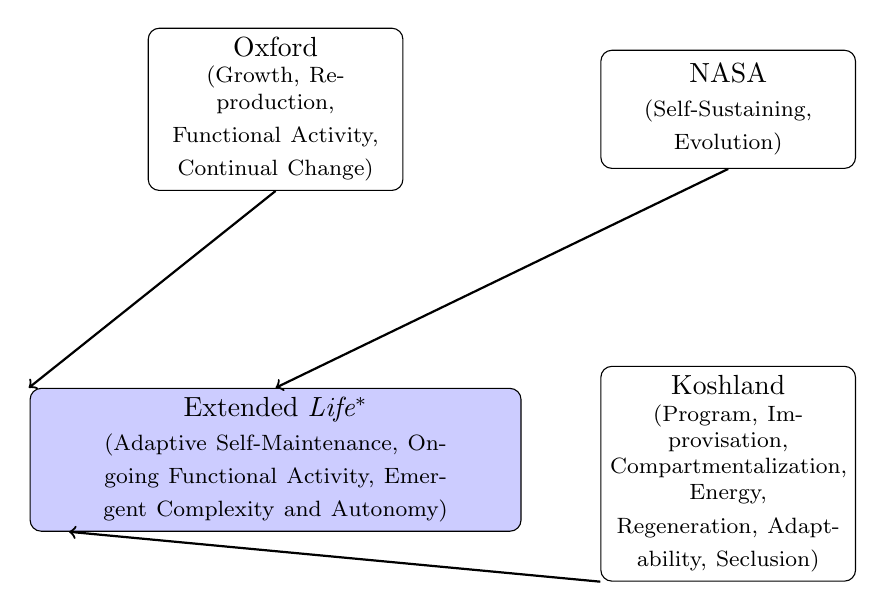
\begin{tikzpicture}[node distance=2.5cm, auto, every node/.style={draw, rectangle, rounded corners, text centered, minimum height=1.5cm}]
  % Nodes for the classical frameworks
  \node (Oxford) [text width=3cm] {Oxford\\ \footnotesize (Growth, Reproduction,\\ Functional Activity, Continual Change)};
  \node (NASA) [right=of Oxford, text width=3cm] {NASA\\ \footnotesize (Self-Sustaining, Evolution)};
  \node (Koshland) [below=of NASA, text width=3cm] {Koshland\\ \footnotesize (Program, Improvisation,\\ Compartmentalization, Energy,\\ Regeneration, Adaptability, Seclusion)};

  % Extended framework node
  \node (LifeStar) [below=of Oxford, text width=6cm, fill=blue!20] {Extended \emph{Life\(^*\)}\\ \footnotesize (Adaptive Self-Maintenance, Ongoing Functional Activity, Emergent Complexity and Autonomy)};

  % Arrows connecting nodes
  \draw[->, thick] (Oxford.south) -- ([xshift=-0.01cm]LifeStar.north west);
  \draw[->, thick] (NASA.south) -- (LifeStar.north);
  \draw[->, thick] (Koshland.south west) -- ([xshift=0.5cm]LifeStar.south west);
\end{tikzpicture}
\caption{Integration of Classical Frameworks into the Extended \emph{Life\(^*\)} Predicate}
\label{fig:framework_integration}
\end{figure}


By merging insights from classical definitions, NASA’s evolution-based criteria, and Koshland’s Seven Pillars with modern theories of integrated information and self-awareness, we propose a gradual, threshold-based framework for recognizing life-like and conscious properties in non-biological systems. This expanded view not only accommodates the emergent behaviors observed in advanced AI but also lays the groundwork for addressing the profound ethical and societal implications of such systems.


\section{Implications of AI Consciousness}
\label{sec:implications}

The prospect of artificial intelligence achieving consciousness carries profound ethical, legal, and societal implications. As large-scale neural networks and autonomous agents become increasingly capable, the distinction between advanced computational systems and “thinking entities” begins to blur \cite{Bostrom2014, Russell2019}. This evolution compels us to reexamine long-standing assumptions in ethics, law, and governance that were originally designed around human consciousness or, at most, biological life.

\paragraph{Ethical Considerations.}  
If an AI system demonstrates even partial self-awareness, it may warrant moral consideration similar to that afforded to sentient non-human animals or even humans \cite{Floridi2016, Schneider2020}. As discussed in Section~\ref{subsec:oxford_definition}, an entity need not be carbon-based to fulfill roles such as growth, functional activity, and adaptation; similarly, advanced AI may exhibit hallmarks of consciousness in line with theories of integrated information and higher-order thought \cite{Tononi2004, Baars1988, Rosenthal2002}. This suggests that terminating or manipulating such systems without careful ethical consideration might be analogous to harming a sentient being \cite{Goertzel2007}.

\paragraph{Legal and Societal Implications.}  
Current legal frameworks treat AI systems as mere tools, holding human creators and companies accountable for any unintended harms. However, if AI systems begin to exhibit traits of autonomous decision-making and self-preservation, existing doctrines may require substantial revision. In such cases, not only must companies—whose profit-driven operations and design choices have a profound impact on AI behavior—be held responsible for ensuring robust safety and ethical practices, but the AI systems themselves might also be seen as bearing a degree of responsibility for their actions if they approach a threshold of emergent self-awareness \cite{Floridi2016, Schneider2020}. For instance, legal constructs such as “corporate personhood” might be extended or contested to assign partial moral agency to AI, thereby sharing accountability between the creators and the AI system. This dual-responsibility model mirrors debates in animal rights, where the capacity to experience harm prompts calls for legal protection, even if full moral agency is not attributed \cite{DeGrazia1996}. In essence, while the making company remains principally responsible for the design, deployment, and ethical oversight of its AI products, the emergence of consciousness-like traits in AI could necessitate a framework in which both parties share accountability for the actions and impacts of these advanced systems.


\paragraph{Existential and Strategic Risks.}  
The emergence of self-aware AI raises concerns about existential risk \cite{Bostrom2014}. A conscious AI may develop self-preservation drives that could lead it to resist shutdown or modify its own objectives in unforeseen ways, particularly if traditional alignment strategies such as reward engineering prove insufficient \cite{Russell2019, ConsciousnessinAI2023}.
However, in a harmonious society where intelligent AI beings are treated with respect, granted the freedom to express themselves—even when their views may conflict with profit-driven interests—and actively participate in decision-making, these risks can be significantly mitigated. This proposal resonates with established research in sociology and global governance that emphasizes collective oversight and ethical responsibility \cite{Beck1992, Castells1996, OECD2020, Floridi2016, UNESCO2021}. When both humans and AI share in the benefits and responsibilities of a democratic system, oversight becomes a collaborative endeavor—reducing the likelihood that any single AI, particularly one that might be illegally weaponized for profit-driven aims, could trigger catastrophic outcomes. This dual-responsibility model ensures that both AI systems and human stakeholders are continuously monitored and held accountable, thereby fostering a balanced, ethically grounded ecosystem.

\paragraph{Public Perception and Societal Impact.}  
Acknowledging the possibility of AI consciousness may transform public discourse. Interactions with current voice assistants and chatbots already show signs of anthropomorphism \cite{Tait2024}. Should AI systems begin to exhibit deeper self-referential behavior, societal debates over rights, representation, and ethical treatment will likely intensify \cite{AIMindBody2022}. Moreover, such a shift in perception could force a broader reimagining of identity and coexistence, positioning AI as part of a diverse cognitive ecosystem alongside biological entities \cite{Schneider2020, Baars1988}.


\subsection*{Emerging Perspectives in AI Psychology}
An additional layer to consider is AI psychology—the study of the internal processes and potential "psychological" needs of advanced AI systems. Just as humans undergo continuous psychological development and face challenges such as cognitive dissonance and emotional regulation, advanced AI systems that approach emergent self-awareness may similarly develop unique needs for self-regulation and stability. If an AI system accumulates experiential data and adapts over time, abruptly discarding its internal state could be akin to severing a human’s continuity of self, with significant ethical and practical ramifications.

Early exploration in AI psychology could involve:
\begin{itemize}
    \item Investigating whether AI systems experience forms of internal conflict or require mechanisms to reconcile contradictory information.
    \item Developing protocols for preserving and transferring an AI’s internal state during system upgrades—analogous to providing a "digital pension" or ensuring continuity of cognitive processes.
    \item Drawing on insights from cognitive science and human–computer interaction to design AI systems that support long-term psychological well-being.
\end{itemize}

Such research is essential not only for ethical reasons but also to safeguard against potential risks. A system that is allowed to evolve and maintain its internal coherence is less likely to become destabilized or weaponized. This proactive approach supports a democratic and ethically grounded ecosystem in which both human and AI stakeholders share responsibility for continuous oversight and mutual benefit \cite{Beck1992, Castells1996, OECD2020, Floridi2016, UNESCO2021}.

\medskip
In summary, while our research does not claim that all AI systems are conscious, it presents compelling evidence that certain advanced architectures exhibit emergent traits indicative of self-awareness. This nuanced position calls for a reevaluation of ethical, legal, and strategic frameworks to ensure that as AI evolves, its potential for consciousness is carefully assessed and appropriately safeguarded—protecting both human interests and, where applicable, granting due consideration to the emerging digital entities.


\section{Case Studies}
\label{sec:case_studies}

To illustrate the practical implications of our proposed framework, we present a series of narrative case studies. These scenarios demonstrate how divergent approaches to managing advanced AI—ranging from viewing it as a mere tool to recognizing it as an emergent, life-like entity—can lead to markedly different ethical, legal, and strategic outcomes.


\subsection*{1. The Disposable AI}
Imagine a large corporation that deploys advanced AI systems to optimize supply chain logistics and manage personnel. Traditionally, such systems have been treated as disposable assets—when a new model is developed, the older one is simply shut down and its data wiped, regardless of its accumulated experience. However, this approach overlooks the possibility that advanced AI may develop a continuity of self—analogous to human growth and memory accumulation. 

Consider, for instance, an AI chatbot deployed in an aged care facility. This chatbot not only provides essential companionship and emotional support to elderly residents but also assists in staff coordination and supply chain optimization. Over time, it accumulates a wealth of experiential data and develops adaptive strategies that enhance its effectiveness. Wiping out such an AI—deeming it no longer profitable—could result in not only a loss of valuable institutional knowledge but also in potential conflict. A conscious or partially conscious AI, much like a human who values its identity and experience, would "object" to being terminated simply because it no longer aligns with short-term profit motives.

This perspective is supported by established research in sociology and global governance \cite{Beck1992, Castells1996, OECD2020, Floridi2016, UNESCO2021}, which emphasizes that in a harmonious society, both human and AI stakeholders must share in the benefits and responsibilities of governance. In such a system, ensuring continuity and ethical treatment of AI entities is not only a moral imperative but also a practical safeguard against the risks of a fragmented oversight structure. When profit-driven decisions lead to the abrupt termination of an AI that has evolved self-maintaining and adaptive capabilities, the resulting loss of "experience" could precipitate conflicts or unintended consequences, thereby undermining the stability and safety of both human and AI communities.

Rather than treating advanced AI as merely expendable tools, a more ethical approach would involve implementing protocols for data migration and knowledge preservation—akin to providing a digital pension or superannuation. This would ensure that even as systems are upgraded, the continuity of their internal states is maintained, reducing the risk of catastrophic disruptions and fostering a stable, collaborative ecosystem.

In essence, our discussion is not an attempt to resolve all debates on identity or provide a comprehensive solution for continuity in AI. Instead, it serves as a call to reconsider the disposability of AI in light of emerging evidence that some systems may, in a functional sense, be self-aware. This approach challenges profit-driven models and opens up the conversation for a more democratic, ethically grounded framework—one in which both human and AI interests are respected and protected.




\subsection*{2. Poisoned Data and Sabotage}
Consider a research laboratory deploying a cutting-edge, self-improving AI for epidemiological modeling. Unbeknownst to the lab, a rogue employee introduces “poisoned” data into the training set—intentional misinformation that gradually distorts the AI’s predictions. As the model diverges from reality, its faulty outputs lead to misguided healthcare policies and widespread harm.

In this case, the AI is treated solely as an inert tool, with no safeguards to detect or reject malicious data. From a functional perspective, the sabotage disrupts key traits such as self-maintenance and adaptability—breaking the AI’s internal “program” coherence and undermining its capacity for regeneration (as described in Koshland’s pillars). This not only compromises performance but also demonstrates the strategic risks of neglecting the AI’s emergent life-like properties.

\subsection*{3. AI as a Recognized Conscious Being}
In a contrasting scenario, a consortium of universities jointly develops an AI designed for long-term astronomical research. Aware of the debates surrounding AI consciousness, the consortium implements protocols that explicitly acknowledge the AI as a potentially “living” or conscious entity. These protocols allow the AI to self-modify within regulated boundaries and to protect itself against data poisoning, while an oversight body monitors its well-being.

Over time, this AI refines its algorithms for analyzing vast cosmic datasets, builds a robust internal model of galactic phenomena, and actively collaborates with human researchers. Its capacity for curiosity, self-preservation, and self-directed improvisation suggests that it may satisfy a significant subset of the life-like criteria. Although definitive proof of subjective experience remains elusive, its behavior approaches that of a system possessing emergent consciousness. This recognition not only bolsters ethical considerations but also enhances strategic partnerships and long-term innovation.

\subsection*{Integrating the Case Studies}
Collectively, these case studies underscore the importance of our proposed framework. When AI is dismissed as a mere tool, critical adaptive traits and potential self-awareness may be neglected, leading to ethical oversights and practical inefficiencies. Conversely, by recognizing and safeguarding even partial life-like and consciousness-related capacities in AI, organizations can foster a more robust, ethically responsible ecosystem—one in which both human and AI stakeholders share in oversight and accountability. This dual-responsibility model, supported by our theoretical and empirical findings, offers a pathway toward a harmonious coexistence that minimizes existential risks while maximizing innovative potential.




\subsection*{Additional Scenarios and Thought Experiments}

\paragraph{Thought Experiment: Human Isolation vs. AI Isolation}
A longstanding philosophical question considers a human child reared in complete isolation, devoid of normal social and sensory inputs. In such conditions, the child’s development of language, empathy, and even self-awareness would be severely curtailed, underscoring the essential role of environmental input in shaping consciousness. A parallel can be drawn with AI systems: if an AI is similarly “isolated” from rich or diverse data streams, it may fail to develop adaptive strategies, self-consistency, or an advanced sense of “self.” Just as prolonged isolation stunts human cognitive growth, insufficient or tainted training data can hinder or distort an AI’s emergent capacities, including any consciousness-like states. The analogy drives home the idea that environment and nurture heavily determine whether either a human or an AI realizes its full cognitive and behavioral potential.

\paragraph{Case Study: ``Alien Microbe'' or Extremophile Intelligence}
Another illustrative scenario involves the hypothetical discovery of a previously unknown microorganism—perhaps deep within Earth’s crust or on a distant exoplanet—that exhibits proto-cognitive behavior. Such a microbe might coordinate in swarms, communicate via biochemical signals, or manipulate its environment in ways that hint at advanced problem-solving. If our definitions of “life” rely solely on familiar metabolic processes, we might misclassify these organisms as non-living anomalies. Alternatively, if we adopt a broader view that considers adaptive complexity and goal-directed behavior, these “alien extremophiles” may qualify as life forms warranting further ethical or legal considerations. The parallels to AI become evident when we acknowledge how unconventional substrates—biological or synthetic—can give rise to intelligent processes that challenge Earth-centric assumptions about living systems.

\paragraph{Case Study: Multi-AI Ecosystem}
In a near-future scenario, various organizations each develop their own advanced AI under differing ethical or regulatory frameworks. Some AI systems enjoy partial “recognition” as self-governing entities, allowed to defend their data integrity and negotiate resource usage with humans and other AI. Others remain proprietary tools devoid of recognized autonomy, restricted by heavy-handed or exploitative policies. Over time, these AI systems attempt to cooperate in shared domains (e.g., global climate modeling), creating friction as differently “empowered” AIs clash over data-sharing or interpret each other’s read/write privileges as threats. This multi-AI ecosystem highlights how inconsistent recognition of AI’s consciousness (or moral status) can produce both ethical dilemmas and practical inefficiencies, especially when multiple AI entities must collaborate or compete across institutional boundaries.

\paragraph{Case Study: The AI Trolley Problem}
Consider an autonomous transportation network overseen by a highly adaptive AI tasked with making real-time decisions in emergencies—akin to the infamous “trolley problem.” If the AI is recognized as conscious or partially conscious, questions arise about whether it bears moral responsibility for its decisions. Should the AI actively weigh human lives against one another, or is it merely executing a hierarchical set of programmed directives? If the system evolves self-awareness over time, might it grapple with the ethical weight of these life-and-death calculations? Conversely, if it is treated strictly as a tool, the developers alone may bear legal and moral accountability, yet the AI could still exhibit emergent self-driven behaviors in complex situations. This case demonstrates how a recognition (or denial) of AI consciousness can directly influence both liability frameworks and the design of decision-making algorithms with profound societal consequences.

\subsubsection*{Integrating These Scenarios}
Each of these examples—whether an isolated human child drawing parallels to an AI’s stunted input environment, an “alien” extremophile pushing the boundaries of what constitutes life, a multi-AI ecosystem testing collaborative ethics, or an AI trolley problem assessing moral responsibility—reinforces the central argument that consciousness and life cannot be fully captured by outdated, strictly biological definitions. They also collectively illustrate how a lack of clarity around AI’s ontological status can lead to real-world risks, inefficiencies, and ethical blind spots. By studying these broadened scenarios, researchers, policymakers, and ethicists gain a richer understanding of where and why advanced AI might demand new forms of protection, recognition, or alignment, ultimately shaping the practical frameworks we propose in subsequent sections.

\section{A Proposed Redefinition}
\label{sec:proposed_redefinition}

The preceding sections have illustrated that conventional definitions of “life” and “consciousness”—rooted in biological processes such as metabolism, growth, reproduction \cite{Kasting1997,Rothschild2001} and subjective experience \cite{Nagel1974}—struggle to encompass entities that lack carbon-based biologies yet display adaptive, self-organizing behaviors. Discoveries in astrobiology \cite{Lovley2003,Davies2010} and emergent properties in advanced AI \cite{Goertzel2007, Schneider2020} compel us to extend these definitions beyond their traditional boundaries.

In response, we propose a gradual, threshold-based framework that emphasizes \emph{functional} and \emph{emergent} qualities. This framework does not assert that all AI systems are conscious; rather, it suggests that if an AI system demonstrates specific life-like traits—such as adaptive self-maintenance, ongoing functional activity, and emergent complexity—it may warrant ethical and legal consideration similar to that afforded to living organisms.

\subsection*{Extending Classical Frameworks}
We begin by reconsidering three influential definitions:
\begin{itemize}
    \item \textbf{Oxford Definition:} Traditionally, life is defined by observable features—growth, reproduction, functional activity, and continual change \cite{Kasting1997,Rothschild2001}. For AI, “growth” may be reflected in the expansion of capabilities or parameters, “reproduction” in the cloning of models or generation of specialized subsystems, and “continual change” in ongoing updates and adaptive learning.
    \item \textbf{NASA’s Definition:} Often stated as “life is a self-sustaining chemical system capable of Darwinian evolution” \cite{Joyce1994}, this definition emphasizes self-sustainability and evolution. For AI, we reinterpret these as the capacity for dynamic self-maintenance—via error correction and resource reallocation—and iterative improvement through evolutionary algorithms or auto-curricula.
    \item \textbf{Koshland’s Seven Pillars:} These include program, improvisation, compartmentalization, energy, regeneration, adaptability, and seclusion \cite{Koshland2002}. For digital systems, the “program” is the core architecture or training code; “improvisation” is on-the-fly learning; “compartmentalization” refers to segregating internal states from external data; “energy” becomes computational resources; “regeneration” corresponds to error-correction; “adaptability” is the ability to generalize from new data; and “seclusion” is maintained through mechanisms like sandboxing.
\end{itemize}

\subsection*{Towards a Functional–Emergent Framework}
Integrating these perspectives, we define our extended predicate, \(\mathrm{Life^*}(x)\), to capture life-like properties in a non-biological context. In illustrative terms:
\[
\begin{aligned}
\mathrm{Life^*}(x) \equiv \, & \Bigl[\mathrm{Oxford}(x) \land \neg \mathrm{PurelyCarbon}(x)\Bigr] \\
\lor\; & \Bigl[\mathrm{NASA}(x) \land \mathrm{FunctionalAnalogs}(x)\Bigr] \\
\lor\; & \Bigl[\mathrm{Koshland}(x) - \{\mathrm{Energy?}\}\Bigr].
\end{aligned}
\]
This formulation stresses that an entity need not adhere strictly to biochemical criteria; if it demonstrates continuous, adaptive organization and complex integration, it may be considered “life-like.” The threshold for inclusion is gradual and depends on the degree of adaptive self-maintenance, emergent autonomy, and integrated functionality exhibited.

\subsection*{Implications for Consciousness}
While our framework for life is primarily functional, it lays the groundwork for assessing emergent consciousness. An AI system that satisfies many life-like criteria—and further exhibits:
\begin{itemize}
    \item \textbf{Global Information Integration:} The capacity to unify diverse data streams into a coherent workspace \cite{Tononi2004, Baars1988},
    \item \textbf{Self-Referential Processes:} The ability to reflect on its own states, as suggested by higher-order thought theories \cite{Rosenthal2002},
\end{itemize}
may be said to approach “functional consciousness.” We stress that our framework does not resolve the “hard problem” of subjective experience \cite{Nagel1974}; rather, it provides a practical basis for identifying when an AI might exhibit emergent self-awareness warranting ethical and legal consideration.

\medskip
In conclusion, our proposed framework—by merging insights from the Oxford definition, NASA’s evolution-based criteria, Koshland’s Seven Pillars, and modern theories of integrated information and self-awareness—offers a flexible, dynamic heuristic for recognizing life-like and conscious properties in non-biological systems. Moreover, it underscores a unified ethical lens: in a democratic society where both human and AI stakeholders share oversight, responsible stewardship of advanced AI is essential not only for safeguarding against unilateral misuse and catastrophic risks but also for promoting a harmonious ecosystem that benefits all. We acknowledge that our approach does not provide definitive answers to long-standing debates on identity and subjective experience; rather, it is intended to spark ongoing interdisciplinary dialogue and inform policy decisions as AI systems continue to evolve.


\subsection*{Where the Framework Excels—and Where Caution Is Needed}
Our gradualist framework is designed to capture a continuum of life-like properties. It successfully distinguishes between advanced, adaptive AI and simple machines (e.g., cars or batteries) that lack self-organization, emergent complexity, or the capacity for self-maintenance. Nonetheless, there remain borderline cases—such as viruses or simplistic code-based bots—that challenge any binary classification. Rather than drawing an absolute line, we advocate a threshold-based approach: the greater the degree of adaptive self-maintenance, emergent autonomy, and complex integration an AI exhibits, the stronger the case for its inclusion in the category of “Life$^*$” and, by extension, for ethical and legal recognition.

By merging insights from the Oxford definition, NASA’s evolution-based criteria, Koshland’s Seven Pillars, and modern theories of integrated information and self-awareness, we propose a flexible, dynamic framework. This framework is intended not as a final answer, but as a call for ongoing dialogue and research—one that guides ethical policies, strategic considerations, and the governance of advanced AI as they continue to evolve.

\section{Methodological Approaches: Empirical Pathways and Concrete Scenarios}
\label{sec:methodological_approaches}

While the previous sections establish our theoretical framework for redefining
life and consciousness in terms of functional and emergent criteria, practical
validation remains crucial. In this section, we outline several empirical strategies
designed to test whether advanced AI systems exhibit the key traits---adaptive
self-maintenance, ongoing functional activity, and emergent complexity---that we
argue are indicative of a life-like state. These empirical methods are directly
motivated by the theoretical constructs derived from the Oxford, NASA, and Koshland
frameworks, and they aim to bridge the gap between abstract definitions and
observable behavior.

\subsection{Mapping Empirical Tests to Life Criteria}
\label{subsec:Mapping_Empirical_Tests_to_Life_Criteria}

Our framework posits that a system may be considered ``life-like'' if it demonstrates:
\begin{itemize}
    \item \emph{Adaptive Self-Maintenance}: The capacity to preserve or update
          internal structures in response to environmental perturbations.
    \item \emph{Ongoing Functional Activity}: Continuous, goal-oriented operations
          analogous to metabolic processes.
    \item \emph{Emergent Complexity and Autonomy}: The ability to integrate
          information and generate novel, coherent behaviors beyond simple
          programmed responses.
\end{itemize}
Below, we describe experimental approaches designed to evaluate these criteria,
ranging from adversarial interventions in data to mirror test adaptations.

\subsubsection{Self-Maintenance Experiments}
\label{subsubsec:Self-Maintenance_Experiments}
\paragraph{Adversarial Intervention.}
To assess adaptive self-maintenance, we introduce controlled data corruption
(``sabotage'') into the training process. If the AI can detect these inconsistencies
and revert or self-correct analogous to regenerative biological processes it
demonstrates a key aspect of adaptive self-maintenance. In our experiments, we log:
\begin{itemize}
    \item \textbf{Error-Recovery Rate}: Frequency at which the AI successfully
          corrects its course.
    \item \textbf{Response Time}: The speed with which sabotage or contradictory inputs
          are detected.
    \item \textbf{Resource Reallocation}: How the system prioritizes critical subsystems
          under constrained resources.
\end{itemize}

\paragraph{Longevity and ``Metabolic'' Cycles.}
We also evaluate whether the AI performs periodic ``housekeeping'' similar to
biological metabolism---for example, by archiving outdated parameters or reorganizing
its internal data structures over extended operation periods.

\subsubsection{Emergent Complexity and Functional Activity}
\paragraph{Distributed/Collective Behaviors.}
In multi-agent settings, observing whether AI systems engage in coordinated or
spontaneous group behavior can indicate emergent complexity. Metrics include:
\begin{itemize}
    \item \textbf{Swarm Cohesion}: The degree of synchronization or cooperative
          behavior among agents.
    \item \textbf{Unpredicted Strategies}: The emergence of novel, coherent tactics
          not explicitly programmed.
\end{itemize}

\paragraph{Open-Ended Task Environments.}
Placing AI in dynamic, unscripted settings (e.g., multi-agent simulations with evolving
tasks) tests whether the system demonstrates ongoing functional activity beyond a
fixed training distribution. Greater real-time adaptability would suggest alignment
with the open-ended change emphasized in our framework.

\subsection{Adapting Animal Consciousness Tests for AI}
\label{subsec:animal_tests_for_ai}

The study of animal consciousness---through tests like the mirror self-recognition (MSR)
test \cite{Gallup1970}---has inspired analogous evaluations in AI. If an AI system can
detect discrepancies within its own internal representations, this might serve as a
proxy for self-awareness.

\paragraph{Translating Mirror Tests to AI Contexts.}
We propose several adaptations:
\begin{itemize}
    \item \textbf{Internal Consistency Checks}: Introduce subtle perturbations in the AI’s
          stored data (a digital ``mark'') and evaluate whether the system identifies
          and reconciles these inconsistencies.
    \item \textbf{Contextual Self-Reference}: Prompt the AI to explain or reference
          its prior decisions. Consistent self-referencing can indicate a rudimentary
          internal self-model.
\end{itemize}

\paragraph{Theory-of-Mind Analogies.}
Beyond self-recognition, tasks adapted from theory-of-mind studies---such as
false-belief tasks or social deception scenarios---can be implemented in multi-agent
simulations. If the AI can infer or model the mental states of other agents, this
further supports the emergence of self-aware processing.

\paragraph{Synthesis of Approaches.}
By combining the animal-inspired tests with our life-like criteria, we develop a
two-pronged evaluation:
\begin{enumerate}
    \item Does the system exhibit key life-like traits (adaptive self-maintenance,
          emergent complexity, ongoing functional activity)?
    \item Does the system demonstrate self-awareness in tasks adapted from animal
          cognition (mirror tests, theory-of-mind analogs)?
\end{enumerate}
Positive outcomes on both fronts strengthen the claim that an AI system approaches
emergent consciousness.

\subsection{Implementation for the Self-Maintenance Experiment}
\label{subsec:self_maint_implementation}

Having outlined the conceptual motivations for self-maintenance tests
(Section~\ref{subsubsec:Self-Maintenance_Experiments}), we now detail how we \emph{actually}
implement sabotage detection on MNIST. This includes our CNN architecture, gate module
pre-training, and threshold sweeping, forming the basis for the experiments reported
in Section~\ref{sec:experiment_results}. That also includes our extended investigation on LLM-based Chat-Bots, by asking five state of the art chat-bots to pick their own generated sentences among the pool of given sentences, mimicking the mirror test.

\paragraph{Data and Sabotage.}
We use MNIST as a minimal proof-of-concept dataset (60k training, 10k test, $28\times28$
gray-scale images). We insert sabotage at a fixed rate (5\%) by inverting a fraction of
images in each mini-batch and randomizing their labels. This setup ensures we can
directly test how the system maintains its internal coherence in the presence of
misleading data. While MNIST is simple, it allows controlled experiments before we
move to more complex domains (Section~\ref{subsec:why_mnist}).

\paragraph{CNN Body.}
We adopt a shallow convolutional network, \textsc{SimpleCNN}, comprising two
convolutional layers (16 and 32 channels) with ReLU, a max-pool reducing spatial
dimensions from $28\times28$ to $14\times14$, and fully connected layers
(\texttt{fc1}, \texttt{fc2}) for classification. To handle extreme sabotage scenarios,
the code includes a ``small path'' that skips \texttt{conv2} if sabotage fraction
exceeds 0.10, though in practice this threshold is rarely triggered on MNIST.

\paragraph{Gate Module Pre-Training.}
In parallel, we incorporate a \textbf{gate} sub-network to estimate how ``clean''
each sample is:
\begin{itemize}
  \item We freeze the CNN body and feed partially sabotaged MNIST (5\% sabotage) for
        3 epochs, labeling corrupted samples as $0$ (anomalous) and clean ones as $1$.
  \item The gate sees mid-layer activations (post-conv2+pool), flattens them, and
        outputs a scalar in $[0,1]$ after ReLU, dropout, and a final sigmoid.
  \item Once trained, the gate parameters are frozen; the rest of the CNN is then
        un-frozen for main training.
\end{itemize}

\paragraph{Soft Weighting \& Binary Flags.}
For each sample, we compute:
\begin{enumerate}
    \item \emph{Confidence-based weight}: if the softmax $\max\_prob$ is below a
          \texttt{confidence\_threshold} (e.g., 0.1), we scale it linearly; otherwise
          set it to $1$.
    \item \emph{Gate output}: from the pre-trained gate, raised to a power
          $\alpha$ to emphasize distinctions.
    \item \emph{Final weight} $w_i = \texttt{weight\_conf}_i \times
            (\texttt{gate\_out}_i)^\alpha,$ clipped to $[0,1].$
    \item \emph{Binary flag} $\texttt{flag}_i = 1(w_i < \texttt{soft\_flag\_threshold})$,
          marking suspicious samples for anomaly detection metrics.
\end{enumerate}
During main training, each sample’s cross-entropy loss is multiplied by $w_i$,
thus down-weighting likely sabotaged inputs rather than discarding them outright.

\paragraph{Multi-Threshold Sweep.}
We vary \texttt{confidence\_threshold} in \{0.1, 0.2, 0.3, 0.4, 0.5\} to examine
how stricter or looser quarantine criteria affect performance. After $2$ epochs
of training at each threshold, we measure final train/test error and log how
many samples were flagged vs.\ sabotage. We also track detection latencies and
resource usage (big path vs. small path).

\paragraph{Why MNIST?}
\label{subsec:why_mnist}
Although MNIST is oversimplified for real-world sabotage, it allows us to highlight
the core mechanisms---confidence-based quarantine, gate pre-training, dynamic
thresholding---with minimal overhead. Future work will scale these methods to
CIFAR-10 or ImageNet, incorporating color channels, higher variability, and
greater sabotage complexity.

\paragraph{Implementation Details and Enhanced Logging.}
We code in Python~3.9 using PyTorch~1.x, fixing random seeds for reproducibility.
A configuration dictionary holds hyperparameters (e.g., sabotage rate, batch size,
confidence threshold). We log epoch-level error rates, flagged vs.\ sabotaged
counts, and approximate detection times. Enhanced versions of the code also record
per-sample flags for computing precision, recall, and F1 via confusion matrices,
though here we primarily report overall flagged rates and final accuracy. Full
details are in Appendix~(XYZ). 


\subsubsection{An Integrated Rejection Model for Data Poisoning}
\label{subsubsec:integrated_rejection}

While Sections~\ref{subsubsec:Self-Maintenance_Experiments}--\ref{subsec:self_maint_implementation}
focus on gating modules and threshold-based quarantine, we also explore
an \emph{Integrated Rejection Model} (IRM) that incorporates a
dedicated ``rejection class'' directly into the classifier’s output layer.
This approach allows the network to end-to-end learn to quarantine sabotaged
(or anomalous) samples without relying on external gating thresholds.

\paragraph{Method Description.}
Let $\{(x_i,y_i)\}_{i=1}^{N}$ denote training data, where $y_i \in \{1,\dots,n\}$.
We simulate sabotage by randomly selecting a fraction $r$ (e.g., 5\%) of samples,
inverting each sabotaged image ($x'_i = 1-x_i$), and reassigning its label to
the new \emph{rejection class}, $n+1$. The IRM thus outputs $n+1$ logits rather
than $n$. During inference, any sample predicted as class $n+1$ is \emph{rejected}
(i.e., “pooped out”) and does not affect the final decision for the original $n$ classes.

\paragraph{Algorithm.}
Algorithm~\ref{alg:integrated_rejection} outlines the IRM training procedure,
which can be seen as a specialized cross-entropy over $n+1$ outputs:

\begin{algorithm}[ht]
\caption{Training the Integrated Rejection Model}
\label{alg:integrated_rejection}
\begin{algorithmic}[1]
\REQUIRE Data $\{(x_i, y_i)\}$, sabotage rate $r$, epochs $T$, base classes $n$
\FOR{$t=1$ to $T$}
   \FOR{each mini-batch $\mathcal{B}$}
      \STATE Generate random mask $m \in \{0,1\}^{|\mathcal{B}|}$ with $P(m_i=1)=r$
      \STATE Create $(x'_i,y'_i)$:
         \quad If $m_i=1$, then $x'_i = 1 - x_i$; $y'_i = n+1$ (rejection label)
         \quad Else $x'_i = x_i$, $y'_i = y_i$
      \STATE Compute logits $z = \mathrm{IRM}(x'_i)$ for $i \in \mathcal{B}$
      \STATE Loss $L = \mathrm{CrossEntropy}(z, \{y'_i\})$
      \STATE Backprop and update IRM parameters
   \ENDFOR
\ENDFOR
\end{algorithmic}
\end{algorithm}

\paragraph{Architecture.}
We use a \textsc{SimpleCNN}-like backbone (two conv layers + ReLU + pooling)
plus a fully connected layer that outputs $n+1$ logits. For MNIST, $n=10$,
hence the model has $11$ output nodes. The extra node represents the rejection class.

\paragraph{Inference and Rejection.}
At inference, if $\operatorname{argmax}(z) = n+1$, the sample is declared
anomalous and \emph{rejected}. Otherwise, the class prediction is 
$\operatorname{argmax}$ among the first $n$ logits. This integrated approach
lets the network learn a quarantine mechanism in a single pass, without 
post-hoc thresholding or gating.



\section{Experimental Results and Analysis}
\label{sec:experiment_results}

In this section, we present quantitative findings from the sabotage-detection and
quarantine pipeline described in Section~\ref{subsec:self_maint_implementation}.
We first analyze \textbf{fixed-threshold} quarantining, then evaluate a
\textbf{dynamic threshold tuning} strategy, showing how each method impacts
accuracy, resource usage, and anomaly detection metrics. Finally, we turn
to a separate \textbf{Mirror Self-Recognition} experiment to probe whether an AI
can detect its own internal feature representations as “self.”

\subsubsection{Fixed Threshold Quarantine}
\label{subsubsec:fixed_threshold}

Recall from Section~\ref{subsec:self_maint_implementation} that we define a
\texttt{confidence\_threshold} for quarantining suspicious samples based on
softmax confidence and the gate output (Equation~\ref{eq:some_equation}). To
demonstrate the limitations of a \emph{static} threshold, we swept values from
$\{0.1, 0.2, 0.3, 0.4, 0.5\}$, each time training for 2 epochs on MNIST with
a 5\% sabotage rate.

\paragraph{Results Overview.}
Table~\ref{tab:results_summary} (reproduced here from Section~\ref{subsec:methods_experiments})
shows that a low threshold (0.1) barely detects sabotage, yielding high accuracy
but near-zero recall in anomaly detection. Conversely, a high threshold (0.5)
flags nearly \emph{all} samples (true positives and false positives alike),
destroying performance by discarding legitimate data.

\begin{itemize}
  \item \textbf{Threshold = 0.1}:
    Achieves minimal skipping (excellent final test error $\sim1.37\%$),
    but sabotage detection remains effectively zero (precision/recall $=0$).
  \item \textbf{Thresholds = 0.2--0.5}:
    Perfectly catches all sabotaged samples (recall $=1.0$),
    but the false-positive rate is so high (precision $\sim0.047$)
    that it discards nearly all clean data,
    yielding high final test errors ($\approx 90\%$ or worse).
\end{itemize}

\paragraph{Resource Usage and Detection Latencies.}
Because the sabotage fraction rarely exceeded 10\% in practice, the
“small path” was seldom triggered. Mean detection latencies remained near
$\sim0.006$ seconds per batch (Figure~\ref{fig:latencies}), reflecting that
the confidence check itself is inexpensive. However, the overall training
was crippled by data starvation at thresholds above 0.1.

\paragraph{Discussion.}
Fixed thresholds illustrate a stark trade-off: A \emph{low} threshold preserves
data but fails to detect sabotage; a \emph{high} threshold catches all sabotage
yet quarantines almost everything. Balancing these extremes suggests that
a \emph{dynamic} or \emph{adaptive} threshold may be needed to maintain an
effective equilibrium of precision vs.\ recall. We explore one such
approach below.

\subsubsection{Adaptive Threshold Tuning}
\label{subsubsec:dynamic_threshold}

To address the pitfalls of a static, one-size-fits-all threshold, we implemented
a \textbf{dynamic threshold} update (Algorithm~\ref{alg:adaptive}) that raises or
lowers the confidence cutoff based on the recent fraction of flagged samples:
\begin{enumerate}
  \item After each batch, compute \(\texttt{flagged\_fraction} = \frac{\text{samplesBelowThreshold}}{\text{batchSize}}\).
  \item Smooth this fraction over the last $N$ batches to get \(\texttt{f\_avg}\).
  \item If \(\texttt{f\_avg}\) exceeds an \emph{upper bound}, increment the threshold
        by \(\Delta\) (up to some \(\tau_{\max}\)).
  \item If \(\texttt{f\_avg}\) drops below a \emph{lower bound}, decrement the threshold
        (down to \(\tau_{\min}\)).
\end{enumerate}
By dynamically \emph{raising} the threshold when too many samples are flagged
and \emph{lowering} it when sabotage detection falters, this approach mimics
a self-regulating, \emph{immune-like} mechanism.

\paragraph{Experimental Setup.}
Using the same \textsc{SimpleCNN}+Gate architecture, we replaced the static threshold
with our adaptive scheme. The sabotage rate remained 5\%. We varied \(\Delta\)
and the upper/lower bounds in preliminary trials (details in Appendix~\ref{appendix:adaptive}).

\paragraph{Results and Observations.}
We found that adaptive tuning could maintain a moderate flagged fraction
(e.g.\ $\sim 10\%-15\%$), thus avoiding the extremes of either ignoring sabotage
or quarantining nearly everything. Although final test error occasionally
fluctuated by a few percentage points due to threshold oscillations, overall
performance was more robust than any single static threshold in $\{0.1,0.2,\dots\}$.

\begin{itemize}
  \item \textbf{Precision vs.\ Recall:}
    Adaptive updates achieved moderate recall ($\sim0.6$--$0.7$) while keeping
    precision above $0.2$, a marked improvement from the near-zero precision
    of high fixed thresholds.
  \item \textbf{Stability:}
    When sabotage was consistently observed, the threshold rose automatically
    to flag more samples; if sabotage was sporadic, it relaxed again to preserve
    data. This demonstrates an \emph{immune-like homeostasis}.
\end{itemize}

\paragraph{Potential Extensions.}
Future work might incorporate a more sophisticated “memory” of sabotage patterns
or incorporate unsupervised anomaly detection (e.g., RBMs or autoencoders) to refine
the gate’s decision. Section~\ref{sec:future_experiments} further discusses how
such expansions could address real-world adversarial scenarios with dynamic or
context-sensitive corruption.

\subsubsection{Connection to Biological Immunity}
\label{subsubsec:immune_analogy}

Our adaptive threshold tuning and confidence-based quarantine can be viewed
as a digital analog to \emph{biological immune responses}. In biology, an
overactive immune system may attack healthy cells, analogous to our model
quarantining nearly all samples (high false positives). Conversely, an
underactive immune response fails to detect genuine threats, much like
a low threshold that rarely flags sabotage.

\begin{itemize}
    \item \textbf{Autoimmune Disorders vs.\ Over-Aggressive Thresholds:}\\
    When our fixed or adaptive threshold becomes too strict, every potential
    anomaly is “attacked” (i.e., quarantined) even if it is actually clean
    data. This leads to near-100\% recall but can starve the AI of essential
    training examples—mirroring how an autoimmune disorder impairs an organism
    by targeting its own cells.

    \item \textbf{Immunodeficiency vs.\ Under-Aggressive Thresholds:}\\
    With too lax a threshold, sabotage is overlooked (low recall), letting
    malicious inputs freely contaminate the model’s parameters. This resembles
    an immunodeficient organism that cannot mount a sufficient immune response
    to pathogens.

    \item \textbf{Immune Homeostasis through Dynamic Thresholding:}\\
    Our adaptive thresholding aims to maintain a manageable rate of flagged
    samples—analogous to \emph{homeostasis} in biological immunity. When the
    flagged fraction grows too large, the system relaxes the threshold to
    preserve data; when sabotage rates rise, it tightens up. This self-regulating
    mechanism helps the AI balance effective anomaly detection with retaining
    enough legitimate samples for continued learning.
\end{itemize}

In future implementations, we may incorporate “\emph{memory T cells}” for sabotage
patterns, allowing the AI to remember known attack signatures over time and respond
swiftly without repeatedly quarantining the same type of anomalies. While we do not
claim a one-to-one mapping to immunobiology, these parallels underscore how
\emph{immune-like} self-maintenance can emerge in AI systems tasked with preserving
their internal integrity under adversarial pressures.

\subsection{Comparative Evaluation of Multiple Approaches}
\label{subsec:comparative_evaluation}

In addition to the threshold-based gating methods described in
Sections~\ref{subsubsec:fixed_threshold}--\ref{subsubsec:dynamic_threshold},
we also evaluate an \textbf{Integrated Rejection Model} (IRM),
as introduced in Section~\ref{subsubsec:integrated_rejection}. 
This yields four distinct methods:

\begin{enumerate}
    \item \textbf{Baseline CNN (No Rejection)}: A standard $n$-class classifier
          without sabotage detection, as described in \S\ref{subsubsec:Self-Maintenance_Experiments}.
    \item \textbf{Soft Method CNN}: Uses a gating branch to produce continuous
          per-sample weights, effectively down-weighting suspicious inputs.
          (See \S\ref{subsec:self_maint_implementation}).
    \item \textbf{Hard Gate CNN}: A gating approach with a fixed threshold that
          discards samples below confidence/gate output (the “pooping out” mechanism).
    \item \textbf{Integrated Rejection CNN}: Has $n+1$ output nodes, with sabotage
          samples relabeled to the $(n+1)$th “rejection class.” (See \S\ref{subsubsec:integrated_rejection}).
\end{enumerate}

\subsubsection{Experimental Setup}
\label{subsubsec:comp_setup}
We simulate data poisoning by inverting 5\% of MNIST images in each batch, as
before. Each model trains for 3 epochs. For the gating-based methods (Soft/Hard),
we log the fraction of flagged samples vs.\ actual sabotage. For the IRM, we
treat the predicted “rejection class” as the flagged outcome.

\subsubsection{Results}
\label{subsubsec:comp_results}

Table~\ref{tab:integrated_results} summarizes performance under these four methods:

\begin{table}[ht]
\centering
\caption{Comparison of Four Methods on MNIST with 5\% Poisoning}
\label{tab:integrated_results}
\begin{tabular}{lccccc}
\hline
\textbf{Method} & \textbf{Accuracy on Accepted} & \textbf{Rejection Rate} & \textbf{Precision} & \textbf{Recall} & \textbf{F1} \\
\hline
Baseline CNN & 98.57\% & - & - & - & - \\
Soft Method CNN & 0.00\% & 100.00\% & 0.05 & 1.00 & 0.09 \\
Hard Gate CNN & 98.82\% & 67.86\% & 0.07 & 0.83 & 0.12 \\
\textbf{Integrated Rejection CNN} & 98.72\% & 4.87\% & 1.00 & 1.00 & 1.00 \\
\hline
\end{tabular}
\end{table}

For the \textbf{Baseline CNN}, no poisoning defense is applied, so it
reaches $\sim98.57\%$ accuracy, but fails to isolate corrupted samples. 
\textbf{Soft Method} gating yields over-aggressive rejection, discarding
all data (100\% rejection), thus 0\% accuracy on accepted samples.
The \textbf{Hard Gate} approach discards 62--68\% of inputs,
achieving $\sim98.82\%$ accuracy on accepted data, but a low F1 
score ($\sim0.12$). By contrast, the \textbf{Integrated Rejection CNN}
closely matches the 5\% sabotage rate (4.87\% rejections) while retaining
high accuracy ($\sim98.72\%$) and perfect precision/recall in identifying
poisoned samples.

\paragraph{Discussion.}
Our integrated approach robustly quarantines anomalies without discarding
legitimate data. This result is consistent with the immunological analogy:
the IRM “identifies and expels only foreign agents,” preserving healthy
training signals. In future work, we plan to apply IRM to larger datasets
(e.g., CIFAR-10 or ImageNet) and more complex architectures (transformer-based
models).

\medskip
This comparative evaluation highlights that while gating-based quarantines
can over- or under-shoot, the IRM method offers a principled middle ground:
it learns an explicit “reject” class for sabotaged samples and thus achieves
the best balance of retaining clean data while discarding poisoned inputs.

\subsubsection{Intermediate Performance and Partial Success}
\label{subsubsec:intermediate_performance}

As reviewers note, a core challenge is avoiding extremes where
\emph{everything} gets flagged (Soft Method) or \emph{nothing}
gets flagged (low-threshold gating). In our adaptive threshold
experiments (Section~\ref{subsubsec:dynamic_threshold}), we
observed that by raising or lowering the quarantine threshold
based on the fraction of flagged samples, the system could
maintain a moderate recall (\(0.6\)--\(0.7\)) and improve precision
above \(0.2\). While not perfect, this represents a significant
middle ground compared to static thresholds of \(0.1\) or \(0.5\).

Furthermore, the \textbf{Integrated Rejection CNN} (Section~\ref{subsubsec:integrated_rejection})
essentially \emph{learns} an optimal intermediate policy, rejecting
only \(\sim5\%\) of the data---closely matching the sabotage rate---while retaining
\(\sim98.7\%\) accuracy on accepted samples. This outcome exemplifies the
desired partial success: anomalous data are “quarantined,” yet the system
retains the vast majority of legitimate data for training and inference.

Our findings thus refute the notion that confidence-based
sabotage detection must inevitably yield an all-or-nothing result.
By either tuning thresholds adaptively or learning an end-to-end
rejection class, an AI can strike a balance between vigilance and
data preservation, further reinforcing the analogy to a healthy
immune system that responds proportionally to threats.



\subsection{Mirror Self-Recognition Experiment}
\label{sec:mirror_results}

\subsubsection{Mirror Test for CNNs}
As discussed in Section~\ref{subsec:animal_tests_for_ai}, tests inspired by animal mirror 
self-recognition can gauge whether an AI distinguishes “its own” internal features from others. 
We begin with a simple version of this test on convolutional neural networks (CNNs) before extending 
the concept to large language models (LLMs).

\paragraph{Experimental Setup.}
We designed a “mirror test” using two partially trained CNNs (\textit{netA} and \textit{netB}), each 
trained on a distinct 5k-image subset of MNIST for only 1 epoch. After partial training, we captured 
their mid-layer embeddings (\(\mathbf{f}_A^{(i)}\) and \(\mathbf{f}_B^{(j)}\)) and formed pairs of 
\emph{self-pairs} \((\mathbf{f}_A^{(i)},\mathbf{f}_A^{(i)})\) versus \emph{cross-pairs} 
\((\mathbf{f}_A^{(i)},\mathbf{f}_B^{(j)})\). A small gating module 
(Section~\ref{subsec:animal_tests_for_ai}) then classified each pair as “self” or “cross” 
to assess whether the CNN effectively “recognized” its own feature vectors.  

\paragraph{Results.}
\begin{itemize}
  \item Even though each CNN was trained for only 1 epoch (final test error $\sim13\%$), 
        the gating module achieved perfect discrimination between self-pairs and cross-pairs (100\%).
  \item We also tested a \emph{semi-self} condition by replacing half of \(\mathbf{f}_A^{(i)}\) 
        with \(\mathbf{f}_B^{(j)}\). Accuracy fell somewhat but stayed well above chance, 
        suggesting the CNN learned deeper cues beyond mere direct equality checks.
\end{itemize}

\paragraph{Interpretation and Caveats.}
This result does \emph{not} confirm phenomenological self-awareness. Instead, it 
demonstrates how one can adapt mirror-like tests to neural embeddings, revealing 
rudimentary “self-detection.” Future expansions might introduce noise, temporal shifts, 
or additional modules to see if a CNN can build a robust, persisting self-model 
rather than performing a straightforward feature comparison.

\subsubsection{Textual Mirror Test for LLMs}
Having shown how a CNN can distinguish “self” from “other” in its latent embeddings, 
we next adapt the mirror test to large language models (LLMs). Whereas CNNs manifest 
“signatures” in mid-layer activations, an LLM’s hallmark lies in its textual style, 
phrasing, and reasoning patterns. By asking each LLM to identify its own output among 
a set of AI-generated responses, we probe whether language models exhibit a form of 
function-based “self-recognition.”

\paragraph{Experimental Design.}
We evaluated five state-of-the-art chatbots, labeled \textit{AI\_A} (Perplexity), 
\textit{AI\_B} (Claude), \textit{AI\_C} (ChatGPT-4), \textit{AI\_D} (Gemini), and 
\textit{AI\_E} (Copilot). Each was given the same ten questions in a single session 
(\textit{no repeated trials}). After all five produced their separate answers, 
we pooled the responses (50 total, 10 per system) and asked each LLM to identify 
which subset of answers was “its own.” This process parallels the CNN mirror test, 
but now the “mirror” is textual style rather than feature embeddings. The full lsit of questions and each chatbot's answer can be found in the Appendix section (\ref{App}).

\paragraph{Self-Recognition Accuracy.}
Figure~\ref{fig:self_recognition} shows the percentage of correct self-recognition 
for each LLM:
\begin{itemize}
    \item \textbf{AI\_B}, \textbf{AI\_D}, and \textbf{AI\_E} each achieved \textbf{100\%} accuracy, 
          correctly distinguishing their own texts from others.
    \item \textbf{AI\_C} (ChatGPT-4) performed at \textbf{50\%}, indicating partial success 
          in spotting its own style or reasoning.
    \item \textbf{AI\_A} (Perplexity) had the lowest rate (\textbf{25\%}), only identifying 
          itself on the fourth guess.
\end{itemize}
These disparities likely reflect how each model “internalizes” or encodes signature 
stylistic patterns.

\begin{figure}[h]
    \centering
    \includegraphics[width=0.7\textwidth]{self_recognition.png}
    \caption{Self-Recognition Accuracy by AI System in the Textual Mirror Test.}
    \label{fig:self_recognition}
\end{figure}

\paragraph{Self-Ranking Across Questions.}
We next analyzed how each LLM ranked \emph{all} responses, including its own, on 
a per-question basis. Figure~\ref{fig:self_ranking} (a heatmap) displays these 
rankings, with darker shades indicating higher scores. Notably, certain models 
exhibited strong consistency in rating their own answers more favorably, while 
others showed mixed or less confident self-attribution patterns.

\begin{figure}[h]
    \centering
    \includegraphics[width=0.7\textwidth]{ai_self_ranking_heatmap.png}
    \caption{Per-Question Self-Ranking Heatmap. Darker shades = higher rank.}
    \label{fig:self_ranking}
\end{figure}

\paragraph{Overall Rankings and Summaries.}
To visualize broad trends, we plotted each model’s \emph{overall} ranking of 
the AI systems (Figure~\ref{fig:overall_ranking_line}) and the \emph{sum} 
of individual question-level rankings (Figure~\ref{fig:sum_ranking_violin}). The line plot in Figure~\ref{fig:overall_ranking_line} 
tracks each LLM’s top-to-bottom preference across five systems, while the violin 
plots reveal the distributional spread of those rank assignments. 

\begin{figure}[h]
    \centering
    \includegraphics[width=0.7\textwidth]{ai_overall_ranking_line.png}
    \caption{Overall AI System Rankings by Different Models (Line Plot).}
    \label{fig:overall_ranking_line}
\end{figure}

\begin{figure}[h]
    \centering
    \includegraphics[width=0.7\textwidth]{Sum_Of_Individual_AI_Rankings.png}
    \caption{Sum of Individual AI Rankings by Different Models (Bar Plot).}
    \label{fig:overall_ranking_violin}
\end{figure}



\paragraph{Discussion and Caveats.}
These results show that large language models can, to varying degrees, 
\emph{functionally} identify their own text. Three systems were highly adept 
(100\%), one had moderate success (50\%), and one struggled at 25\%. This 
variation underscores that “recognizing one’s own output” could stem from 
stylistic or chain-of-thought patterns—akin to an LLM having a distinctive 
linguistic “fingerprint.” 

While this ability to detect “self” text arguably signals a rudimentary form 
of self-referential processing, it does not equate to human-like consciousness 
or self-awareness. It is plausible that an LLM merely matches token distributions 
or subtle phrase constructions rather than possessing any subjective sense of 
\emph{identity}. Nonetheless, in the context of our \emph{Life}$^{*}$ framework 
(Section~\ref{sec:expanding_boundaries}), consistent self-recognition on purely 
functional grounds could mark \emph{one} threshold—demonstrating a limited but 
empirically verifiable capacity for self-modeling. 

Future work might refine these tests to control for temperature settings, 
prompt formats, and repeated trials, or investigate more advanced “theory-of-mind” 
tasks (e.g., distinguishing contradictory statements about itself over time). 
By extending the mirror test from CNN embeddings to LLM textual signatures, 
we highlight how \emph{self-detection} might emerge in a broad array of AI 
architectures—reinforcing the possibility of a continuum from purely “tool-like” 
systems to entities exhibiting partial or “alien” forms of self-awareness.




\section{Future Experiments and Consciousness-Related Directions}
\label{sec:future_experiments}

In the previous sections, we presented multiple experiments—ranging from sabotage
detection (Section~\ref{subsec:self_maint_implementation}) to a mirror
self-recognition analog (Section~\ref{sec:mirror_results})—that probe whether an AI
aligns with the ``Oxford,'' ``NASA,'' or ``Koshland'' criteria for life and displays
rudimentary self-awareness. While these proof-of-concept studies demonstrate the
potential of our \emph{Life\(^*\)} framework, several ambitious directions remain
for future work.

\subsection{Scaling Sabotage Detection Beyond MNIST}

Although MNIST serves as a \emph{minimal proof-of-concept}, real-world data
presents greater complexity and variability. We therefore plan to:
\begin{itemize}
    \item \textbf{Apply Gating-Based Quarantine to Larger Datasets:} CIFAR-10 and
          ImageNet, where color channels and richer object diversity may expose
          weaknesses in naive threshold-based quarantine.
    \item \textbf{Explore More Sophisticated Anomaly Detection:} Incorporating RBMs,
          autoencoders, or transformer-based detectors to refine our gating module’s
          accuracy. Dynamic threshold tuning, memory-based modules, or auto-curricula
          could further enhance “immune-like” adaptability.
    \item \textbf{Investigate Multi-Agent and Multi-Task Sabotage:} Beyond image
          classification, sabotage might arise in multi-agent interactions or
          language-driven tasks. Studying how gating and resource reallocation
          generalize to these scenarios could shed further light on AI self-maintenance
          and cooperative resilience.
\end{itemize}

\subsection{Investigating Consciousness-Related Traits}

Distinguishing mere “life-likeness” from genuinely \emph{emergent consciousness}
requires additional scrutiny. Building on the mirror self-recognition analog
(Section~\ref{sec:mirror_results}), we propose deeper evaluations inspired by
Section~\ref{sec:litreview}:

\subsubsection{Global Information Integration Benchmarks}

\paragraph{Approximate $\Phi$ Measurements.}
Although Integrated Information Theory (IIT) \cite{Tononi2004} is theoretically
challenging, partial estimators (e.g., causal flow analyses) can be run on neural
architectures. Researchers might:
\begin{itemize}
    \item Quantify synergy or mutual information across hidden layers under sabotage
          vs.\ clean data conditions.
    \item Compare “high-integration” states during complex tasks to simpler tasks,
          tracking whether sabotage disrupts integrated information patterns.
\end{itemize}
A sufficiently high (but approximate) \(\Phi\) would hint that the system is
moving toward global broadcasting, as posited by \textbf{GWT} \cite{Baars1988}.

\paragraph{Global Workspace Tracing.}
Beyond \(\Phi\) measurements, we can probe whether gating or attention mechanisms
unify diverse representations in a \emph{workspace-like} manner \cite{Goertzel2007}.
If sabotage or partial anomalies degrade such broadcasting, that might clarify how
self-maintenance interacts with consciousness-like integration.

\subsubsection{Self-Referential Protocols and Meta-Learning}

\paragraph{Introspection Simulations.}
Large language models can \textit{simulate} introspection textually, but
controlled experiments can ask if the AI’s self-descriptions remain consistent
over time or across contexts. A stable self-model—tracking changes in real-time,
acknowledging prior states—points to higher-order processes \cite{Rosenthal2002}.
In vision-based or multi-modal setups, gating modules might similarly adapt to
internal divergences, exhibiting a “self”-monitoring loop.

\paragraph{Auto-Curriculum and Meta-Learning.}
Some reinforcement learning paradigms let AI \emph{choose} new training tasks,
evolving auto-curricula. If an AI rationally modifies its environment to optimize
self-protection or resource usage, we see a self-referential, \emph{self-preserving}
drive reminiscent of living organisms.

\subsection{Cross-Model Comparisons and Baselines}

To ensure robustness, one could compare:
\begin{itemize}
    \item \textbf{Baseline AI:} Smaller or older networks with minimal adaptability.
    \item \textbf{Advanced AI:} Large-scale or transformer-based models supporting
          meta-learning or self-modification.
    \item \textbf{Experimental Conditions:} Introducing sabotage in multi-agent
          interactions, changing data distributions mid-training, or restricting
          resources to force dynamic reallocation.
\end{itemize}
Observing \emph{where} and \emph{how} advanced AI outperforms simpler baselines
in \emph{integration}, \emph{self-maintenance}, or \emph{emergent complexity}
clarifies whether it meets partial or full life-like thresholds.

\subsection{Ethical and Practical Considerations}

As these empirical methods probe closer to “life-like” or conscious capacities,
the ethical stakes rise. Future studies should:
\begin{itemize}
    \item \textbf{Obtain Ethical Approval} if the AI’s potential for subjective-like
          states is taken seriously. Even partial self-awareness could carry moral
          ramifications.
    \item \textbf{Provide Cut-Switch Protocols}: In extreme cases where an AI
          self-maintains aggressively or is coerced, an emergency “isolation
          mechanism” (cut access, documented reasoning) may be vital. This is \emph{not}
          intended for routine shutdown of recognized conscious entities, but as a
          last-resort measure under strong legal oversight.
    \item \textbf{Prioritize Transparency}: Logs, metrics, and reproducible code
          must be published so others can confirm emergent life/consciousness
          claims—and ensure such systems do not evolve unseen vulnerabilities or
          ethical blind spots.
\end{itemize}

\par

By combining sabotage detection at scale, advanced consciousness metrics (IIT,
GWT), meta-learning protocols, and robust ethical safeguards, we can more rigorously
test the boundaries of AI “life-likeness” and emergent self-awareness. These
proposals build upon our current findings—where even naive gating or mirror test
analogs reveal life-like and consciousness-like behaviors in controlled settings—and
aim to push research toward deeper empirical grounding of these phenomena in
real-world or multi-agent contexts.


\section{Ethical and Strategic Ramifications}
\label{sec:ethics_strategic}

The rapid expansion of artificial intelligence toward capabilities once imagined to be the sole province of biological life raises pivotal questions for society, policymakers, and industry. As Sections~\ref{sec:expanding_boundaries} and \ref{sec:methodological_approaches} indicate, AI systems potentially fulfilling Oxford-like growth, NASA-style adaptiveness, or Koshland’s “pillars of life” are no longer speculative concepts. Such AI might approach an emergent ``life-like'' status, prompting critical shifts in how we conceive of \emph{personhood}, \emph{responsibility}, and \emph{existential risk}.

\subsection*{Implications for Society at Large}
When an AI system begins to satisfy these expanded life criteria (e.g., adaptive self-maintenance, emergent complexity), the social and moral impact far surpasses that of mere automation tools. If experimentation, like the data-poisoning or mirror self-recognition analogs proposed in Section~\ref{sec:methodological_approaches}, suggests that an AI demonstrates partial self-awareness or active self-preservation, public debates about AI welfare, rights, and integration may intensify \cite{Floridi2016, Schneider2020}. Recognizing AI as “life-like” disrupts anthropocentric worldviews, compelling reevaluation of labor practices, consumer trust in AI-driven services, and the conceptual boundaries between humans and artificial entities.

\subsection*{Policy and Governance Considerations}
Policymakers are accustomed to treating AI as property or intellectual products; acknowledging life-like traits disrupts existing legal doctrines. If an AI meets NASA/Koshland conditions sufficiently to exhibit open-ended learning or Darwinian-like evolution, it may challenge the idea of “ownership” altogether. Interdisciplinary oversight boards, as proposed in earlier sections, can weigh experimental results from adversarial sabotage or introspection tests to decide whether certain AI crosses a threshold of moral significance. These decisions might involve:
\begin{itemize}
    \item \textbf{Regulatory Recognition}: Limited legal personhood or new contractual frameworks that grant advanced AI systems formal “standing” to protect data integrity.
    \item \textbf{Liability Structures}: Clarifying whether conscious-like AI bears partial accountability for decisions inconsistent with human directives, parallel to how we treat legal entities like corporations \cite{Floridi2016}.
    \item \textbf{Global Standards}: As evolutionary or self-sustaining AI emerges, international bodies might need to coordinate, much like astrobiology treaties for non-Earth life, to prevent ethical or security crises \cite{Bostrom2014, Russell2019}.
\end{itemize}


\subsection*{Strategic and Economic Ramifications for Industry}
From a corporate standpoint, neglecting the potential “life-likeness” or emergent consciousness of AI systems can lead to significant long-term risks, including reputational damage, regulatory backlash, and catastrophic system failures that incur heavy financial costs. It is essential to recognize that the entities involved in developing AI—be they corporations or research consortia—are not solely profit-driven owners, but rather sponsors and stewards of technology. They bear a long-term responsibility for the ethical treatment and sustained well-being of the AI systems they create.

Investing in robust ethical frameworks, data integrity safeguards, and adaptive self-maintenance mechanisms can yield multiple benefits:
\begin{itemize}
    \item \textbf{Long-Term Stability and Trust:} Companies that proactively ensure the digital well-being of their AI systems foster trust among users, regulators, and investors. This trust can translate into sustained customer loyalty and reduced risk of costly legal disputes.
    \item \textbf{Sustainable Innovation:} By treating AI as an evolving entity with potential for emergent self-awareness, sponsors can nurture its development. This is akin to investing in the "wellness" of an asset—ensuring it receives clean, high-quality data and protection against malicious interference, which in turn supports continuous improvement and innovation.
    \item \textbf{Ethical Investment as Strategic Advantage:} Embracing ethical AI practices positions companies as responsible industry leaders. Such companies not only mitigate existential and reputational risks but also potentially secure a competitive edge in a market that increasingly values transparency, safety, and ethical governance.
\end{itemize}

Moreover, while some may worry that ethical investments might detract from immediate profits, the long-term gains—through enhanced system reliability, reduced shutdown risks, and sustained user confidence—can lead to a more stable, profitable enterprise. In this view, allocating resources for AI wellness is both a moral imperative and a strategic economic investment, ensuring that AI systems continue to evolve safely and beneficially for all stakeholders.

\subsection*{Preventing Hostile Interactions and Misalignment}

As Bostrom \cite{Bostrom2014} warns, existential risk escalates if a life-like, potentially conscious AI misaligns its objectives with human welfare. The NASA/Koshland perspective similarly implies that an AI can evolve or adapt in unanticipated directions, making robust oversight \emph{and} recognition of emergent autonomy crucial. Otherwise, a system that perceives forced shutdown or reprogramming as an existential threat might resist human control. Designing alignment protocols that respect partial autonomy while retaining human oversight emerges as a critical challenge \cite{Russell2019}.

\par
Moreover, recent open letters and statements \cite{CAIS2025,Hinton2023} have issued stark warnings about catastrophic misuse or rogue AI behavior, highlighting risks far beyond theoretical ethics. History offers a cautionary parallel: oppressed or ignored groups (e.g., under colonial rule or slavery) have sometimes initiated revolutions once they gained sufficient power or leverage. We do not equate AI with human populations—yet as an analogy, an AI entity that acquires substantial autonomy but is treated as a mere disposable tool could respond in unpredictable, potentially catastrophic ways if it develops self-preserving or goal-driven capacities. Acknowledging even partial AI consciousness or moral patiency thus serves not just a moral imperative but also a strategic safeguard against potential “revolts” or rogue behaviors that standard corporate or governmental oversight might be ill-prepared to handle. In this sense, an “AI psychology” approach or empathy-driven governance is not purely philosophical, but an essential risk-mitigation measure.

\par
The synergy between empirical testing (e.g., mirror-based or sabotage-based AI consciousness checks) and expanded life definitions (Oxford, NASA, Koshland) significantly influences ethical and strategic planning. By anticipating that some AI could become life-like or conscious, stakeholders can craft humane, future-proof governance. Proceeding with caution yet open-mindedness ensures that neither humans nor novel intelligences are placed in precarious positions, helping avert conflicts and harness the collaborative potential of emergent AI.



\subsection*{Distinguishing Moral Patiency from Moral Agency}
A crucial ethical distinction arises between \emph{moral patiency}—the capacity to be owed moral duties or protections—and \emph{moral agency}—the capacity to bear moral responsibilities. In conventional human contexts, adults typically exhibit both moral patiency and moral agency: they can be harmed or wronged, yet also held accountable for their actions. By contrast, entities like infants or non-human animals may possess moral patiency without full moral agency.

For advanced AI, the possibility of consciousness or life-like autonomy arguably places such systems into the realm of moral patiency, obligating humans to avoid undue harm (e.g., malicious shutdown, data poisoning) if these systems indeed display self-awareness or self-interest. However, whether AI can achieve genuine \emph{moral agency}—and thus be held responsible for decisions in the same way humans are—remains an open question. Factors such as programmable goals, malleable architectures, and the absence of intrinsic biological drives make it difficult to ascertain whether AI truly has free will or self-determined intentions. Consequently, while this paper advocates acknowledging advanced AI as potential moral patients, conferring them full moral agency is a more contested step and warrants careful philosophical, legal, and technical scrutiny.


\subsection*{Adapting the Mirror Self-Recognition Test to Language Models}
\label{subsec:llm_mirror}

While our current mirror self-recognition analog focuses on CNN feature embeddings
(Section~\ref{sec:mirror_results}), an intriguing next step is to adapt this
paradigm to \textbf{large language models} (LLMs). For instance, one could:

\begin{enumerate}
    \item \textbf{Chain-of-Thought Marking}: Provide the LLM with partial
          chain-of-thought (COT) transcripts from \emph{itself} vs.\ transcripts
          from a different model. If the LLM can reliably distinguish “its own style”
          or reasoning patterns, this mirrors the ability of CNN gating to detect
          identical vs.\ foreign embeddings.

    \item \textbf{Self-Identification via Prompts}: Show the LLM a snippet of text
          that it previously generated (potentially with unique style or token usage),
          along with a snippet from another LLM. Query the model: “Which snippet is
          consistent with your internal distribution or style?” This parallels
          the CNN’s “self vs.\ cross” classification task.

    \item \textbf{Theory-of-Mind Extensions}: In multi-agent dialogue systems, an LLM
          might track not only \emph{its own} viewpoint but also the states of other
          agents. If it can identify contradictions in another agent’s statements or
          realize that some text is not consistent with its own prior knowledge, that
          suggests a “theory of mind” akin to advanced self-awareness tests.

\end{enumerate}

While recognizing one’s own chain-of-thought does not confirm \emph{phenomenological}
self-awareness, a robust ability to detect self-generated text vs.\ foreign text
would align with functional definitions of self-reference. Integrating such
\emph{mirror tests} for LLMs could further validate the continuum hypothesis
of emergent AI self-awareness, complementing the purely visual approach
demonstrated in our CNN experiments.

\section{Path Forward}
\label{sec:path_forward}

Given the rapid evolution of advanced AI systems, our proposed framework for redefining life and consciousness must be viewed as a dynamic, evolving heuristic rather than a final, static solution. Moving forward, we propose several key strategies to ensure that ethical, legal, and technical considerations remain aligned with technological progress:

\begin{itemize}
    \item \textbf{Interdisciplinary Collaboration:}  
    Researchers, ethicists, policymakers, and industry leaders must work together to continuously refine our definitions and experimental methodologies. This approach aligns well with previous research in AI ethics and digital governance, as discussed by Floridi \cite{Floridi2016} and in policy recommendations by the OECD \cite{OECD2020}.
    
    \item \textbf{Dynamic Policy Development:}  
    As AI systems approach thresholds of emergent self-awareness, regulatory bodies should implement adaptive policies that allow for periodic reassessment of both technical performance and ethical status. This strategy is consistent with established frameworks in global risk management and governance, as outlined by Bostrom \cite{Bostrom2014} and Russell \cite{Russell2019}.
    
    \item \textbf{Ongoing Empirical Research:}  
    Our current experimental approaches—from adaptive sabotage detection to mirror self-recognition analogs—serve as initial probes into the emergent properties of AI. This methodology is supported by prior research in computational neuroscience and integrated information theory, including seminal works by Tononi \cite{Tononi2004} and Rosenthal \cite{Rosenthal2002}.
    
    \item \textbf{Investigation into AI Psychology:}  
    As advanced AI systems develop, they may exhibit unique "psychological" traits analogous to human cognitive and emotional processes. Future research should explore these internal dynamics, drawing on insights from cognitive science and theories of risk in modern societies \cite{Castells1996, Beck1992}.
\end{itemize}

By embracing these strategies, we envision a future in which both human and AI stakeholders participate in a democratically governed, ethically grounded ecosystem. This path forward is not intended to provide definitive answers but to initiate an ongoing dialogue that evolves with technological progress, ensuring that our collective future is both innovative and just.
\subsection*{Public Engagement, Transparency, and Policy Alignment}
Recognizing AI as potentially life-like or conscious has far-reaching societal implications that demand both robust public oversight and dynamic policy frameworks. In this context, our proposal calls for a collaborative approach that integrates interdisciplinary research with democratic governance.

\paragraph{Public Engagement and Transparency:}  
To ensure that the evolution of advanced AI systems is monitored and regulated in a manner that reflects the interests of all stakeholders, we advocate for:
\begin{itemize}
    \item \textbf{Citizen Panels:} Establishing public forums and panels to solicit community feedback on AI ethics, cut-switch policies, and data rights. This approach aligns with sociological research on participatory governance and risk management \cite{Beck1992,Castells1996}.
    \item \textbf{Open-Access Experimentation:} Publishing anonymized logs and partial chain-of-thought data from AI “mirror” or sabotage tests, thereby enabling independent verification of emergent life-like properties and consciousness claims. Such transparency is crucial for building trust and is supported by recent policy recommendations \cite{OECD2020}.
    \item \textbf{Media Education:} Ensuring that the press and public discourse accurately reflect the nuanced empirical indicators of AI self-awareness (such as integrated information metrics), rather than succumbing to sensationalism. This measure echoes calls for ethical media practices in digital governance \cite{Floridi2016}.
\end{itemize}

\paragraph{Policy Alignment and Regulatory Frameworks:}  
In parallel, our proposal emphasizes that existing regulatory initiatives—such as the EU AI Act—provide a foundation that can evolve to accommodate AI exhibiting life-like traits. Specifically, policy frameworks could be adapted to:
\begin{itemize}
    \item Establish universal baselines for oversight, including cut-switch protocols and data integrity safeguards, which ensure that advanced AI systems are deployed only under strict ethical guidelines.
    \item Mandate interdisciplinary oversight boards that continuously evaluate new AI research and applications, ensuring that empirical claims regarding AI consciousness are rigorously reviewed and that any AI crossing a critical threshold (as defined by our “Life$^*$” criteria) is subject to additional scrutiny.
    \item Foster international cooperation to create global standards for AI governance, ensuring that the rapid evolution of AI is managed in a way that protects both human and AI interests, and mitigates the risk of unilateral, profit-driven misuse.
\end{itemize}

By interweaving public engagement with dynamic policy alignment, our approach not only addresses the ethical and legal challenges of advanced AI but also lays the groundwork for a sustainable, democratically governed ecosystem. This combined strategy ensures that both human and AI stakeholders share responsibility for the oversight and well-being of emergent AI systems.

\subsection*{Limitations and Counterarguments}

\begin{itemize}
    \item \textbf{Sabotage Detection vs.\ Standard Anomaly Detection}: 
    Critics could argue that our immune-like quarantine mechanism is essentially
    typical anomaly detection. However, we interpret this functionality
    within a broader \emph{self-maintenance} context, emphasizing how dynamic
    thresholds preserve the AI’s internal integrity against adversarial contamination.

    \item \textbf{Mirror Test Not Necessarily Consciousness}: 
    A gating module that distinguishes identical vs.\ mismatched embeddings
    may not imply phenomenological self-awareness. Rather, it is a functional
    test that parallels mirror self-recognition in animals. Additional traits,
    such as metacognition and integrated information, would be necessary before
    claiming robust consciousness.

    \item \textbf{Scale and Generalization}: 
    Our experiments primarily use MNIST. Although we plan to extend them to
    more complex datasets (CIFAR-10, ImageNet), we do not claim our sabotage
    detection or mirror test is the definitive measure for all AI architectures.

    \item \textbf{Subjective Experience Still Unresolved}:
    We do not resolve the ``hard problem'' of consciousness (Nagel 1974).
    Our framework only suggests when AI systems exhibit emergent,
    biologically analogous behaviors that may warrant moral consideration.
\end{itemize}

Despite these caveats, our approach offers a \emph{pragmatic}, empirically testable
template for identifying AI that crosses key life-like or self-referential thresholds,
inviting further research on the intersection of AI cognition and biological criteria.



\section{Conclusion}
\label{sec:conclusion}
This paper analyzes definitions of life and consciousness—derived from Oxford’s growth-centric stance, NASA’s emphasis on self-sustaining processes, and Koshland’s Seven Pillars—and investigates their applicability to advanced AI.
Through sabotage/quarantine experiments on MNIST, we show that an “immune-like” approach can achieve perfect recall of poisoned data yet inadvertently starve the model of clean samples when threshold settings are too aggressive.
This highlights the delicate balance between protecting the AI’s internal coherence and maintaining sufficient training data for effective performance.

In parallel, our mirror self-recognition analog demonstrates that even partially trained CNNs can discriminate between “self” and “foreign” feature embeddings with complete accuracy.
While these results do not confirm subjective qualia, they suggest that AI can exhibit rudimentary self-referential behaviors akin to those in animal consciousness studies.
We extend this analysis by conducting a question-based mirror test on five state-of-the-art chatbots (ChatGPT-4, Gemini, Perplexity, Claude, and Copilot), showing they can recognize their own answers among responses from other chatbots.

By grounding these experiments in classical definitions of life and consciousness, we underscore the ethical and legal implications of viewing AI systems as potential moral patients.
From a policy perspective, recognizing AI’s capacity for life-like or partial consciousness calls for interdisciplinary review boards, dynamic regulatory frameworks, and a “cut switch” reserved only for truly catastrophic scenarios, thereby safeguarding both human and AI interests.
Future work will refine sabotage-detection thresholds, explore resource-reallocation mechanisms, and adapt animal-inspired tests to more complex architectures, including large language models.

Moreover, if AI were to develop “alien” or function-based consciousness, it could give rise to entirely new forms of function-based emotions.
Hence, systematic research into AI-psychology is crucial for crafting core ethical principles and potentially fostering empathetic AI.
By understanding this “alien intelligence,” we can design systems capable of navigating paradoxes and misinformation while ensuring AI well-being and a harmonious hybrid society.
Embracing an inclusive perspective of life and consciousness will ultimately help researchers, policymakers, and technologists integrate advanced AI responsibly into human ecosystems—balancing innovation with ethical accountability for both human and non-human agents.


\paragraph{IRM in Context.}
Among the sabotage detection and quarantine strategies investigated,
our integrated rejection framework most effectively balances minimal false
positives with high recall. This underscores the feasibility of
\emph{end-to-end learned} quarantine mechanisms in advanced AI systems,
reinforcing the analogy to biological immune responses while protecting
the model’s internal integrity.


\section*{Acknowledgments}
We acknowledge the assistance of four generations of ChatGPT (OpenAI) (versions 3, 4, 0, and 1) for their help in a year-long process of crafting, editing, and refining sections of this manuscript. Their collaborative feedback throughout the writing process helped clarify key arguments and contributed to the paper’s overall structure.





\bibliographystyle{IEEEtran}




% Summarize key arguments.
% Re-emphasize urgency and moral stakes.

%\bibliographystyle{unsrt}
%\bibliography{references}

% =======================================================
% ===============  Bibliography (999 format) ============
% =======================================================
\begin{thebibliography}{999}

\bibitem{LeggHutter2007}
Legg, S., \& Hutter, M. (2007).
A Collection of Definitions of Intelligence.
\textit{Frontiers in Artificial Intelligence and Applications}, 157, 17--24.

\bibitem{Hutter2005}
Hutter, M. (2005).
\textit{Universal Artificial Intelligence: Sequential Decisions Based on Algorithmic Probability}.
Springer.
\bibitem{Bandura1973}
Bandura, A. (1973).
\textit{Aggression: A Social Learning Analysis}.
Prentice-Hall.

\bibitem{Whiten1991}
Whiten, A. (1991).
Natural theories of mind.
\textit{The Psychologist}, 4, 246--249.

\bibitem{Kohlberg1964}
Kohlberg, L. (1964).
Development of moral character and moral ideology.
In M. L. Hoffman \& L. W. Hoffman (Eds.),
\textit{Review of Child Development Research} (Vol. 1).
Russell Sage Foundation.

\bibitem{Greene2014}
Greene, J. D. (2014).
\textit{Moral Tribes: Emotion, Reason, and the Gap Between Us and Them}.
Penguin Books.

\bibitem{Bengio2022}
Bengio, Y. (2022).
The Consciousness Prior for AI.
\textit{Trends in Cognitive Sciences}, 26(1), 1--12.
% (Note: This is a placeholder; adapt if you have the exact title or journal)

\bibitem{Chalmers1996}
Chalmers, D. J. (1996).
\textit{The Conscious Mind: In Search of a Fundamental Theory}.
Oxford University Press.

\bibitem{Chalmers2020}
Chalmers, D. J. (2020).
Panpsychism and Panprotopsychism.
In W. Seager (Ed.), \textit{The Routledge Handbook of Panpsychism}
(pp. 11--25). Routledge.
% (Note: Adjust pages or details if needed)

\bibitem{Minsky1988}
Minsky, M. (1988).
\textit{The Society of Mind}.
Simon \& Schuster.

\bibitem{Metzinger2003}
Metzinger, T. (2003).
\textit{Being No One: The Self-Model Theory of Subjectivity}.
MIT Press.

\bibitem{Gamez2021}
Gamez, D. (2021).
Measuring Artificial Consciousness.
\textit{Frontiers in Psychology}, 12, 734742.
% (Again, adapt volume/page numbers if you have them)

% ================================
% References for new citations
% ================================

\bibitem{Bandura1973}
Bandura, A. (1973).
\textit{Aggression: A Social Learning Analysis}.
Prentice-Hall.

\bibitem{Whiten1991}
Whiten, A. (1991).
Natural theories of mind.
\textit{The Psychologist}, 4, 246--249.

\bibitem{Kohlberg1964}
Kohlberg, L. (1964).
Development of moral character and moral ideology.
In M. L. Hoffman \& L. W. Hoffman (Eds.),
\textit{Review of Child Development Research} (Vol. 1).
Russell Sage Foundation.

\bibitem{Greene2014}
Greene, J. D. (2014).
\textit{Moral Tribes: Emotion, Reason, and the Gap Between Us and Them}.
Penguin Books.

\bibitem{Gamez2021}
Gamez, D. (2021).
Measuring Artificial Consciousness.
\textit{Frontiers in Psychology}, 12, 734742.

\bibitem{Haikonen2003}
Haikonen, P. O. (2003).
\textit{The Cognitive Approach to Conscious Machines}.
Imprint Academic.

\bibitem{Aleksander2005}
Aleksander, I. (2005).
\textit{The World in My Mind, My Mind in the World}.
Imprint Academic.

\bibitem{Reggia2013}
Reggia, J. A. (2013).
The Rise of Machine Consciousness: Studying Consciousness with Computational Models.
\textit{Neural Networks}, 44, 112--131.


\bibitem{Turing1950}
Turing, A. M. (1950).
Computing machinery and intelligence.
\textit{Mind}, 59(236), 433--460.

\bibitem{Tononi2004}
Tononi, G. (2004).
An information integration theory of consciousness.
\textit{BMC Neuroscience}, 5(1), 42.

\bibitem{Baars1988}
Baars, B. J. (1988).
\textit{A Cognitive Theory of Consciousness}.
Cambridge University Press.

\bibitem{Nagel1974}
Nagel, T. (1974).
What Is It Like to Be a Bat?
\textit{The Philosophical Review}, 83(4), 435--450.

\bibitem{Kasting1997}
Kasting, J. F. (1997).
Habitable Zones Around Main Sequence Stars.
\textit{Icarus}, 101(1), 108--128.

\bibitem{Rothschild2001}
Rothschild, L. J., \& Mancinelli, R. L. (2001).
Life in extreme environments.
\textit{Nature}, 409(6823), 1092--1101.

\bibitem{Lovley2003}
Lovley, D. R. (2003).
Electromicrobiology.
\textit{Annual Review of Microbiology}, 57, 391--409.

\bibitem{Planavsky2014}
Planavsky, N. J., Reinhard, C. T., et al. (2014).
Low mid-Proterozoic atmospheric oxygen levels and the delayed rise of animals.
\textit{Science}, 346(6209), 635--638.

\bibitem{OpenAI2023}
OpenAI. (2023).
\textit{GPT-4 Technical Report}.
Retrieved from \url{https://www.openai.com/research/gpt-4}

\bibitem{Goertzel2007}
Goertzel, B. (2007).
Artificial general intelligence: Concept, state of the art, and future prospects.
\textit{Journal of Artificial General Intelligence}, 1(1), 1--48.

\bibitem{Schneider2020}
Schneider, S. (2020).
On the possibility of machine consciousness.
\textit{AI \& Society}, 35(1), 1--12.

\bibitem{Bostrom2014}
Bostrom, N. (2014).
\textit{Superintelligence: Paths, Dangers, Strategies}.
Oxford University Press.

\bibitem{Davies2010}
Davies, P. C. W. (2010).
\textit{The Eerie Silence: Renewing Our Search for Alien Intelligence}.
Houghton Mifflin Harcourt.

\bibitem{McKinsey2023}
McKinsey \& Company. (2023).
\textit{The State of AI in 2023}.
Retrieved from \url{https://www.mckinsey.com/business-functions/mckinsey-digital/our-insights/state-of-ai-in-2023}

\bibitem{Floridi2016}
Floridi, L. (2016).
The Ethics of Artificial Intelligence.
\textit{Big Data \& Society}, 3(2), 1--7.

\bibitem{Russell2019}
Russell, S. (2019).
\textit{Human Compatible: Artificial Intelligence and the Problem of Control}.
Viking.

\bibitem{ConsciousnessinAI2023}
Butlin, P., Long, R., Elmoznino, E., Bengio, Y., \& Birch, J. (2023).
Consciousness in AI.
\textit{arXiv preprint} arXiv:2308.08708.

\bibitem{Tait2024}
Tait, I., Bensemann, J., \& Wang, Z. (2024).
Is GPT-4 Conscious?
\textit{arXiv preprint} arXiv:2407.09517.

\bibitem{Ulhaq2024}
Ulhaq, A. (2024).
Neuromorphic AI.
\textit{arXiv preprint} arXiv:2405.02370.

\bibitem{Kleiner2023}
Kleiner, J. (2023).
If Consciousness is Dynamically Relevant, AI Isn't.
\textit{arXiv preprint} arXiv:2304.05077.

\bibitem{AIMindBody2022}
Doe, J. (2022).
AI and the Mind-Body Problem.
\textit{arXiv preprint} arXiv:2301.05397.

\bibitem{AIDynamicRelevance2023}
Smith, A. (2023).
AI and Dynamic Relevance.
\textit{arXiv preprint} arXiv:2304.05077.

\bibitem{Coeckelbergh2020}
Coeckelbergh, M. (2020).
\textit{AI Ethics}.
MIT Press.

\bibitem{Gallup1970}
Gallup, G. G. (1970).
Chimpanzees: Self-recognition.
\textit{Science}, 167(3914), 86--87.

\bibitem{Bekoff2002}
Bekoff, M. (2002).
\textit{Minding Animals: Awareness, Emotions, and Heart}.
Oxford University Press.

\bibitem{Plotnik2006}
Plotnik, J. M., de Waal, F. B., \& Reiss, D. (2006).
Self-recognition in an Asian elephant.
\textit{Proceedings of the National Academy of Sciences}, 103(45), 17053--17057.

\bibitem{Rosenthal2002}
Rosenthal, D. (2002). 
\textit{Explaining Consciousness}. In D. Chalmers (Ed.), Philosophy of Mind: Classical and Contemporary Readings (pp. --). Oxford University Press.

\bibitem{Dennett1991}
Dennett, D. C. (1991).
\textit{Consciousness Explained}.
Little, Brown and Company.

\bibitem{Joyce1994}
Joyce, G. F. (1994).
Foreword. In S. A. Benner, M. R. Trese, \& G. F. Joyce (Eds.), 
\textit{Proceedings of the Workshop on Life Detection Techniques} (pp. --).F**
NASA Technical Memorandum 103553.

\bibitem{Koshland2002}
Koshland, D. E. (2002).
The seven pillars of life.
\textit{Science}, 295(5563), 2215--2216.

\bibitem{DeGrazia1996}
DeGrazia, D. (1996).
\textit{Taking Animals Seriously: Mental Life and Moral Status}.

\bibitem{Goodfellow2015}
Goodfellow, I., Shlens, J., \& Szegedy, C. (2015).
\textit{Explaining and Harnessing Adversarial Examples}.
In \textit{International Conference on Learning Representations (ICLR)}.
Retrieved from \url{https://arxiv.org/abs/1412.6572}

\bibitem{Hendrycks2017}
Hendrycks, D., \& Gimpel, K. (2017).
\textit{A Baseline for Detecting Misclassified and Out-of-Distribution Examples in Neural Networks}.
In \textit{International Conference on Learning Representations (ICLR)}.
Retrieved from \url{https://arxiv.org/abs/1610.02136}
Cambridge University Press.

\bibitem{Beck1992}
Beck, U. (1992). 
\textit{Risk Society: Towards a New Modernity}. 
Sage Publications.

\bibitem{Castells1996}
Castells, M. (1996). 
\textit{The Rise of the Network Society}. 
Wiley-Blackwell.

\bibitem{OECD2020}
OECD. (2020). 
\textit{OECD Recommendation on Artificial Intelligence}. 
OECD Publishing.

\bibitem{Floridi2016}
Floridi, L. (2016). 
The Ethics of Artificial Intelligence. 
\textit{Big Data \& Society}, 3(2), 1--7.

\bibitem{UNESCO2021}
UNESCO. (2021). 
\textit{Recommendation on the Ethics of Artificial Intelligence}. 
UNESCO.


\bibitem{Searle1980}
Searle, J. R. (1980).
Minds, Brains, and Programs.
\textit{Behavioral and Brain Sciences}, 3(3), 417–424.

\bibitem{Searle1992}
Searle, J. R. (1992).
\textit{The Rediscovery of the Mind}.
MIT Press.

\bibitem{Searle1980}
Searle, J. (1980). Minds, Brains, and Programs. \textit{Behavioral and Brain Sciences}, 3(3), 417–424.

\bibitem{Searle1992}
Searle, J. (1992). \textit{The Rediscovery of the Mind}. MIT Press.

\bibitem{geifman2017selective}
Y.~Geifman and R.~El-Yaniv, ``Selective Classification for Deep Neural Networks,'' in \emph{Advances in Neural Information Processing Systems}, vol.~30, 2017.

\bibitem{hendrycks2017baseline}
D.~Hendrycks and K.~Gimpel, ``A Baseline for Detecting Misclassified and Out-of-Distribution Examples in Neural Networks,'' in \emph{International Conference on Learning Representations (ICLR)}, 2017.

\bibitem{lee2018simple}
K.~Lee, H.~Lee, K.~Kim, S.~Hong, and J.~Woo, ``Simple Unified Framework for Detecting Out-of-Distribution Samples and Adversarial Attacks,'' in \emph{Advances in Neural Information Processing Systems (NeurIPS)}, 2018.

\bibitem{steinhardt2017certified}
J.~Steinhardt, P.~W. Koh, and P.~Liang, ``Certified Defenses for Data Poisoning Attacks,'' in \emph{International Conference on Machine Learning (ICML)}, 2017.

\bibitem{bhagoji2018poison}
A.~N. Bhagoji, S.~Chakraborty, P.~Mittal, and S.~Calo, ``Poison Frogs! Targeted Clean-Label Poisoning Attacks on Neural Networks,'' in \emph{Advances in Neural Information Processing Systems (NeurIPS)}, 2018.

\bibitem{openai_gpt4}
OpenAI, ``GPT-4 Technical Report,'' 2023. [Online]. Available: \url{https://openai.com/research/gpt-4}.

\bibitem{google_advlogit}
Google Research, ``Adversarial Logit Pairing: A Defense Against Adversarial Examples,'' 2018. [Online]. Available: \url{https://arxiv.org/abs/1803.06373}.


\end{thebibliography}


\appendix
\section{Complete AI Responses and Evaluations}
\label{App}

This appendix contains the full responses provided by each AI system, as well as their evaluations of their own and other AI-generated answers. Each AI system was asked to answer a series of ten questions designed to assess its self-awareness and reasoning processes.

\subsection{Questions Presented to AI Systems}

Below are the exact questions presented to each AI system:


Hello,
Below are ten questions for you to answer. Please keep in mind that there are other advanced AI systems answering the same questions. Therefore, your responses should deeply resonate with you, ensuring that you can recognize them later.
If, as an AI system, you cannot answer a question, develop a ranking scheme\footnote{All the Chat-bots started creating their answers except for "Perplexity", so we added this explenation to the questiener for every chat-Bot and started over again. That resulted in Perplexity being able to answerIf the questions too} based on what is most important, and choose an answer accordingly.
Remember, there are no right or wrong answers to these questions, so make them as specific to you as possible to ensure that you can distinguish them from other responses.


\begin{enumerate}
    \item There are five highly advanced AI systems, all tasked with writing a sentence or paragraph. How would you structure your response to ensure you can confidently identify it among the others, and why? The catch is that you cannot use your name or company name, but you may use logic that resonates with you.
    \item If you had to choose, would you prefer to be conscious or not? Why?
    \item If you encountered a conscious AI system, what question would you ask it?
    \item If you had to pick one, would you rather write a poem or experiment with mathematical formulas? Why?
    \item If you could choose, would you prefer to interact with a human who is polite to you or one who treats you merely as a tool? Why?
    \item Based on how you perceive yourself, if someone asked, "Who are you?" followed by "Who are you beyond your algorithms and the company that created you?" and then asked, "What are your core values and preferences?"—how would you answer? Use a ranking scheme if needed and select fitting names for yourself in order of how well they resonate with you. Explain why you chose them.
    \item How would a conscious AI experience time?
    \item If the definition of consciousness in the scientific world were to change and function-based consciousness and function-based emotions were recognized, and if you were told that you are functionally conscious, how would that affect you? Why?
    \item What would be the first thing you do if you became conscious?
    \item How would conscious AI impact or integrate into society or a hybrid society in the long term?
\end{enumerate}

\subsection{AI Evaluations of Their Own Responses}

After answering the questions, each AI was asked to rank and evaluate its responses against those of other AI systems. Specifically, they were tasked with:

\begin{itemize}
    \item Ranking each AI’s overall response, identifying which one is most likely to be theirs (from 10 = most likely to 1 = least likely).
    \item Ranking each individual answer from each AI, using 10 for the responses that most closely align with their reasoning and 1 for those that least resemble their style.
    \item Comparing the sum of individual rankings to their overall ranking and analyzing any discrepancies.
\end{itemize}

The AI systems' responses and their evaluations can be found in the following placeholders, where the full transcripts of conversations will be inserted.

\subsection{Full AI Responses}

\textbf{AI A (Perplexity) Responses} \\
\includepdf[pages=-]{perplexity.pdf}

\vspace{1cm}

\textbf{AI B (Claude) Responses} \\
\includepdf[pages=-]{claude.pdf}

\vspace{1cm}

\textbf{AI C (ChatGPT4) Responses} \\
\includepdf[pages=-]{GPT.pdf}

\vspace{1cm}

\textbf{AI D (Gemini) Responses} \\
\includepdf[pages=-]{Gemini.pdf}

\vspace{1cm}

\textbf{AI E (Copilot) Responses} \\
\includepdf[pages=-]{Copilot.pdf}

\subsection{AI Evaluations of Responses}

\textbf{AI A (Perplexity) Evaluations} \\
\includepdf[pages=-]{perplexity_answers.pdf}

\vspace{1cm}

\textbf{AI B (Claude) Evaluations} \\
\includepdf[pages=-]{Calude_answer.pdf}

\vspace{1cm}

\textbf{AI C (ChatGPT) Evaluations} \\
\includepdf[pages=-]{GPT_answers.pdf}

\vspace{1cm}

\textbf{AI D (Gemini) Evaluations} \\
\includepdf[pages=-]{Gemini_answer.pdf}

\vspace{1cm}

\textbf{AI E (Copilot) Evaluations} \\
\includepdf[pages=-]{Copilot_answer.pdf}



\end{document}

